\documentclass[a4paper,notitlepage]{article}
\usepackage{latexsym}
\usepackage{graphicx}
\usepackage{color}
\usepackage{array}
\usepackage{multirow}
\usepackage{hyperref}
\usepackage{wasysym}
\usepackage{verbatim}
\usepackage{enumerate}
\addtolength{\oddsidemargin}{-.875in}
\addtolength{\evensidemargin}{-.875in}
\addtolength{\textwidth}{1.75in}

\renewcommand\labelitemi{\tiny$\bullet$}

\hypersetup{
    bookmarks=true,         % show bookmarks bar?
    unicode=false,          % non-Latin characters in Acrobat�s bookmarks
    pdftoolbar=true,        % show Acrobat�s toolbar?
    pdfmenubar=true,        % show Acrobat�s menu?
    pdffitwindow=false,     % window fit to page when opened
    pdfstartview={FitH},    % fits the width of the page to the window
    pdftitle={My title},    % title
    pdfauthor={Author},     % author
    pdfsubject={Subject},   % subject of the document
    pdfcreator={Creator},   % creator of the document
    pdfproducer={Producer}, % producer of the document
    pdfkeywords={keyword1} {key2} {key3}, % list of keywords
    pdfnewwindow=true,      % links in new window
    colorlinks=true,       % false: boxed links; true: colored links
    linkcolor=blue,          % color of internal links
    citecolor=green,        % color of links to bibliography
    filecolor=blue,      % color of file links
    urlcolor=cyan           % color of external links
}

\begin{document}

%title
\begin{center}
\noindent { \huge \bfseries LUX Xenon Sampling System Procedure}
\end{center}

%Document Information
\noindent { \large \bfseries Document Approvals}

\noindent
\begin{tabular}{|p{2.25in}|p{1.5in}|p{2.25in}|}
\hline
System & Original Author & Date \\
\hline
\multirow{2}{*}{LUX Xe Sampling} & \multirow{2}{*}{Attila Dobi} & \multirow{2}{*}{11/07/11} \\
 & & \\
\hline
Current Responsible Author & Date & Signature\\
\hline
\multirow{2}{*}{Jon Balajthy} & \multirow{2}{*}{05/14/2014 - present} & \multirow{2}{*}{on twiki} \\
 & & \\
\hline
Reviewer & Date & Signature \\
\hline
\multirow{2}{*}{Nicole Larson} & \multirow{2}{*}{11/08/2012} & \multirow{2}{*}{on twiki} \\
& & \\
\hline
\multirow{2}{*}{Patrick Phelps} & \multirow{2}{*}{11/13/2012} & \multirow{2}{*}{on twiki} \\
& & \\
\hline
\multirow{2}{*}{Blair Edwards} & \multirow{2}{*}{11/25/2013} & \multirow{2}{*}{on twiki} \\
& & \\
\hline
\multirow{2}{*}{Dan McKinsey} & \multirow{2}{*}{04/08/2014} & \multirow{2}{*}{on twiki} \\
& & \\
\hline
\multirow{2}{*}{Rachel Mannino} & \multirow{2}{*}{11/26/2013} & \multirow{2}{*}{on twiki} \\
& & \\
\hline
\multirow{2}{*}{David Taylor} & \multirow{2}{*}{03/26/2014} & \multirow{2}{*}{on twiki} \\
& & \\
\hline
\multirow{2}{*}{Markus Horn} & \multirow{2}{*}{03/31/2014} & \multirow{2}{*}{on twiki} \\
& & \\
\hline
\multirow{2}{*}{Aaron Manalaysay} & \multirow{2}{*}{11/26/2013} & \multirow{2}{*}{on twiki} \\
& & \\
\hline
\multirow{2}{*}{Martha White} & \multirow{2}{*}{05/09/2014} & \multirow{2}{*}{on twiki} \\
& & \\
\hline
\end{tabular}
\\

% Document Revision History
\noindent { \large \bfseries Revision Record}

\noindent
\begin{tabular}{|m{0.5in}|p{2.75in}|p{2.75in}|}
\hline
Revision & Description & Author(s) \& Date \\
\hline
0 & Initial Release & Attila Dobi 11/07/11 \\
\hline
1&Automation Upgrade & Attila Dobi 10/09/12 \\
\hline
2&Automation Upgrade Comments & Attila Dobi 11/13/12 \\
\hline
3&Walkthrough Comments & Attila Dobi 12/03/12 \\
\hline
4&Comments from RO, RK, EB & Attila Dobi 04/30/13 \\
\hline
5&Sampling Xenon Storage Bottles& Attila Dobi 11/26/13 \\
\hline
6&LN Fill Update and DT's comments & Attila Dobi 2/12/14 \\
\hline
7&Xe SB sampling update & Attila Dobi 3/26/14  \\
\hline
8&SAM automation upgrade & Jon Balajthy 5/14/14 \\
\hline
9&Hardware upgrade and Calibration & Jon Balajthy 1/1/15 \\
\hline
 & & \\
\hline
 & & \\
\hline
\end{tabular}
\\

%Environment Definitions
\newenvironment{safe}
{\noindent \color{blue} \begin{tabular}{p{0.75in} @{} p{5.05in}} \\ Hazard Analysis: &}
{\\ \color{black} \end{tabular}}
\newenvironment{risk}
{\noindent \color{red} \begin{tabular}{p{0.75in} @{} p{5.05in}} \\ Operation Risk: &}
{\\ \color{black} \end{tabular}}

\newpage
\tableofcontents
\newpage

%Content

\section{Introduction}
\subsection{Purpose}
The purpose of this document is to guide the user through the process of sampling xenon from the LUX circulation system and analyzing the xenon purity with the coldtrap/RGA method. 

\section{Prerequisites}
\subsection{Skills and Training}
This work requires cryogenics training. HS5030-W "Pressure and Cryogen Safety"
This work will be performed by a Sampling System Expert, to be trained by Attila Dobi.

\subsection{Permits and Authorizations}
Work shall only be completed as authorized by the shift manager.

\subsection{Equipment}
\begin{itemize}
	\item 4 L transfer Dewar with handle
	\item Cooler (for storing liquid nitrogen)
	\item Cryo-gloves
	\item Face shield
	\item Safety Glasses
	\item Lab-jack for supporting cooler
	\item Liquid nitrogen supply with delivery hose	
	\item Portable O2 monitor
\end{itemize}

\subsection{Hazard Mitigation}\label{HazMit}

\begin{tabular}{|m{1.75in}|m{4.5in}|}

\hline 
Hazard & Mitigation \\

\hline 

High Pressure Gas &
\begin{itemize} 
\item All operators have completed HS5030-W, Pressure/Cryogen Safety. 
\item Burst disk set at 41.1 psig (BDCT1) prevents dangerous overpressure in the coldtrap.
\item All components of the system have been pressure tested prior to operation \href{http://teacher.pas.rochester.edu:8080/wiki/pub/Lux/InternalProcedures/luxcriticalprocedure004.pdf;rev=7}{Pressure Test Procedure}
\item Only a fixed amount of xenon will ever be cryopumped into the coldtrap. At most a 0.5 L volume at 3 atm, the maximum pressure in the LUX xenon system, of xenon will be introduced into a 1.0L volume. Engineering controls are built in so that the maximum pressure in the coldtrap will be 1.5 atm, after warming the xenon ice. Since the LUX xenon system can not exceed 4 bar of pressure, without blowing a burst disk, the maximum amount of xenon that can be transferred to the sampling volume is 4 atm in 0.5 L. When expanded into the entire sampling system volume of 2.5 L the resulting pressure is 1.5 atm.  In case of accidental overpressure a bust-disk set to 41.1 psig will relieve the pressure in the coldtrap plumbing.
\end{itemize} \\

\hline

Oxygen Deficiency Hazard (ODH) & \begin{itemize}
\item Oxygen monitors alert personnel to oxygen deficiencies 
\item Inert gases used are only asphyxiants, not toxic. 
\item Closed system reduces asphyxiation hazard; consult \href{http://teacher.pas.rochester.edu:8080/wiki/pub/LuxSafety/OxygenDeficiencyHazards/LUX_LN_ODH_Underground_LdV_2012.pdf}{ODH analysis} for details 
\item Quantity of nitrogen gas and liquid-nitrogen is well below amount need to create oxygen deficiency hazard. Four Liters of Liquid nitrogen will be used to cool the coldtrap. 4 L of LN can expand suddenly to 2800 L of gaseous nitrogen at room temperature. This is less than 0.2\% of the air volume of the Davis cavern.
\item \href{http://teacher.pas.rochester.edu:8080/wiki/pub/LuxSafety/OxygenDeficiencyHazards/LUX_LN_ODH_Underground_LdV_2012.pdf}{ODH analysis} completed and shown that ODH is zero. \end{itemize}\\

\hline

Cryogen Safety & \begin{itemize} 
\item All operators have completed HS5030-W, Pressure/Cryogen Safety. 
\item Personal protective equipments(PPE) such as cryo-gloves, safety glasses, and face shield protect operators from exposure to cryogenic liquid. They will be located by the SRV.
\item The coldtrap consists of 316 S.S. (stainless steel) plumbing, with VCR and conflat connections, which have been pressure tested.
\end{itemize} \\

\hline

Administrative Locking & \begin{itemize}
\item For covering and locking valves in this procedure see operations procedure 36 \href{http://teacher.pas.rochester.edu:8080/wiki/pub/Lux/InternalProcedures/OP36-AdministrativeLocking.pdf}{Administrative Locking}.
\end{itemize}\\
\hline

\end{tabular}

\subsection{Lessons Learned}

\begin{itemize}
\item{RGA overpressure burnout in August 2013.}

Before the sampling algorithm had completed the user clicked a button on slow control to start a new sample. Specifically, the logic had gotten to the stage where SAM is waiting to confirm that the cold trap has warmed up and that the xenon is ready to be pumped away or recovered to the SRV. The sampling system Logic began the pre sampling process in parallel to the pump out process exposing the RGA temporarily to an atmosphere of xenon causing the filament and electron multiplier to burn out.
The way the slow control backend is set up multiple instances of a C script can run in parallel when a front end command is sent.
The problem was fixed by modifying the logic. All user inputs for the``Sampling System Master Control" are disabled until the analysis algorithm has completed and until all reported sampling errors are cleared by the user.
As long as the user follows the procedures the code will do the rest.

\item{Hanging hose ejecting from sampling Dewar during LN fill.}

There have been two instances of the SRV vent line's flex hose ejecting from the sampling system Dewar at the start of the LN fill. High pressure can build up in the LN fill line so when starting the fill there is a possibility that the hose will jolt initially.
This has been address with CP13 version 6.
Mitigated by removing the cover of the Dewar, and placing the Dewar directly under the flex hose (bend as little as possible).
Also we can contain the flex hose to prevent it from swinging around.
The correct response for the operator is to hit the ''Refill Stop" button, wait for the line to stop venting and place the hose back in the Dewar.

\item{SRV recovery procedure.}

It was pointed out that when recovering the sampled xenon to the SRV the high pressure lines should first be opened to the cold SRV prior to opening the vales to the low pressure side. No incidents ever occurred because the pressure in the lines are always checked prior to shorting the low and hight pressure plumbing , this is just good practice.

\end{itemize}
\newpage


\section{Filling the Sampling System's Dewar in the Lower Davis}
\label{Section:3}

\begin{safe}
A cryogen is used in this procedure. Wear PPE including cryo-gloves, safety goggles, and face shield when handling cold cryo-hose fittings and pouring liquid nitrogen. Avoid cuffs and wear proper shoes that cover the toes. Before filling the 4 L transfer Dewar assemble materials, Check that SRV vent line ready to deliver LN (Liquid Nitrogen), Sampling system is ready for LN.  Notify others in the area of impending LN fill. Assure vent line is adequately contained by Dewar that hose whip will not kick the hose out of the Dewar.  Don PPE: Cryo-gloves, safety glasses, face shield, oxygen monitor. Do not place the Dewar lid on Dewar, leave the Dewar open to allow pressure relief. Cuffs that could trap liquid should not be worn when working with LN.  Before using an oxygen monitor, the operator should test if the device is operational.  A simple test is to hold breath for several seconds, then slowly ($>$15 seconds) exhale near the sampling port.  If monitor does not alarm and reads $<$19.5\% do not use. Assure others (non-operators) are out of the area.  The SRV LN Panel is about 2 m from SRV Vent Line and 4 L Dewar. Observe filling of 4 L Dewar from a distance at least 3' away.  Listen for alarms and check personal and fixed oxygen monitors.  If unexpected event occurs during filling or oxygen levels drop to $<$19.5\%: Stop Fill by pushing "Stop Fill" button on the SRV LN Panel and leave the area (it is sufficient to take the stairs up to the upper davis). While filling the 4 L transfer Dewar there is a cryogen hazards to the users and others in the lower Davis, near the SRV. LN Splashes,a spill, or overflow could cause the floor to get slippery and cause oxygen deficiency. Check that the area in lower Davis is clear before transporting the 4 L Dewar to the sampling system. Before pouring LN, check floor and area around the cold trap Dewar for equipment that might be adversely affected by an LN spill.  Pour slowly at start, especially if Dewar is warm.
\end{safe}

\begin{risk}
When starting the fill of the sampling system's Dewar there is a chance that the hanging hose of the SRV vent line could be ejected from the Dewar, due to elevated pressure in the LN fill line. If this occurs stop the flow of LN by pressing the ``Refill STOP" on the SRV LN Panel. See Figure \ref{fig:LN_BOX} for a photo of the SRV LN BOX. The SRV vent line is near an oxygen monitor by the SRV and a LN spill during the filling of the sampling system Dewar may set it off. If the oxygen alarm is set off evacuate the area. Before beginning a LN fill check that the LN percentages of both the SRV and TS are greater than 52\%, displayed on the SRV LN system panel. This is done in order to ensure that the SRV vent line will be free for the next 5 minutes. If either of them are reading less than 52\% then wait until the automated LN system refills them. The coldtrap is a cryopump vessel which could potentially accumulate an amount of xenon which could overpressure when the xenon ice warms up. A burst disk set to 41.1 psig will relieve a overpressure in the coldtrap system plumbing. 
\end{risk}

This section describes the process of filling the 4 L transfer dewar form the SRV vent line and then transferring its contents to the Sampling System's cold trap dewar. Note, the Dewar is to be replaced every six months.

\begin{enumerate}
\item Before beginning check the usage data on the sampling system's Dewar. If the last replacement was over six months ago then replace the Dewar and label the new starting date.
\item On the LN system panels check that the LN percentages of both the SRV and TS are greater than 52\%. This is done in order to ensure that the SRV vent line will be free for the next 5 minutes. If either of them are reading less than 52\% then wait until the automated LN system refills them.
\item Push the button labeled ``Refill SmpSys" on the SRV LN Panel. This will time out the SRV vent for 600 seconds. (Note: You can either use the touch screen interface or the physical button on the LN box).
\item Don Cryogen PPE: Cryo-gloves, safety glasses, face shield. Take the clip tested, functioning oxygen monitor (stored in the LUX office) close to your breathing zone.
\item Place the 4L Dewar (larger white Dewar) into the 95 L S.S. pot located at the SRV vent line.
\item \label{hose_in_Dewar} Adjust the vent line such that the 4 L Dewar is directly underneath the SRV vent line. Do not place the lid on the sampling system's Dewar, leave it open.
\item Push the button labeled ``Refill SmpSys" again. If the line is warm then at first only nitrogen gas will vent from the line. 
\item If the SRV vent hose is ejected from the sampling system Dewar due to an overpressure in the line press the ``Stop Fill" button." Wait for the line to stop venting and return to Step \ref{hose_in_Dewar}.
\item After 5-10 minutes, depending on the initial line temperature, the flow of LN through the SRV vent line will begin at a rate of about 3 l/min. See Figure \ref{fig:LN_BOX} for a photo of the SRV LN BOX.
\item When the sampling system's Dewar is nearly full (about 2 minutes), stop the fill by pushing the ``Refill STOP" on the SRV LN Panel. Once the ``Stop Fill" button is pressed LN will continue to flow for about 30 seconds, wait until the flow stops. See Figure \ref{fig:LN_BOX} for a photo of the SRV LN BOX.
\item There is a 2 minute timer on the Sampling System LN fill that will shut off the flow of LN, the timer begins when LN line temperature drops below -180 C. If you still need to top off then restart the fill by pressing the button labeled ``Refill SmpSys"again (press twice). And then stop the fill by by pushing the ``Refill STOP". Remember, once the ``Stop Fill" button is pressed LN will continue to flow for about 30 seconds.
\item If the LN fill fails to stop, or in the event of an emergency hit the RED ``Emergency Stop" button on the LN panel. Then see \href{http://teacher.pas.rochester.edu:8080/wiki/pub/Lux/InternalProcedures/LUXCriticalProcedure015.pdf}{LN System Procedure}
\item Check that the floor of the lower Davis is clear of obstacles or workers. Lift the Dewar by handle and carry over to sampling system.
\item After a sample has been drawn, pour the LN from the 4 L Dewar into the cold trap Dewar. Before pouring LN, check floor and area around the cold trap Dewar for equipment that might be adversely affected by an LN spill.  Pour slowly at start, especially if Dewar is warm.
\item Completion: Return 4 L Dewar to storage near the SRV vent line and log activity in the LUG.


\end{enumerate}


\section{Using the Automated Sampling System}
\label{sec:main}

\begin{safe}
Cryogen and pressure hazards mitigated as noted in Section 2.4. A cryogen is used in this procedure. Wear PPE including cryo-gloves, safety goggles, and face shield when handling cold cryo-hose fittings and pouring liquid nitrogen. Avoid cuffs and wear proper shoes that cover the toes. Use a portable O2 monitor during LN transfer to ensure the O2 concentration is above 19.5\%.
\end{safe}

\begin{risk}
The coldtrap is a cryopump vessel which could potentially accumulate an amount of xenon which could overpressure when the xenon ice warms up. A burst disk set to 41.1 psig will relieve a overpressure in the coldtrap system plumbing.
\end{risk}

\begin{table}[h!]
\begin{center}
\begin{tabular}{|c|c|c|c|c|c|}
\hline
Sample Location & VA & VB & VC & VB/VC Initial State & Pressure to Watch \\ \hline
Getter Input  & CV37 & CV34 & CV35 & Open & PT-C15 \\ \hline
Getter Output & CV76 & CV74  & n/a & Open & PT-C20\\ \hline
Detector Return & CV11 & CV8 & n/a & Open & PT-C1 \\ \hline
PMT Purge Line & CV9 & CV7 & n/a & Open & PT-D41, PT-D4\\ \hline
Recirc Pump Inlet & CV60 & CV61 & n/a & Closed & PT-C15 \\ \hline
Storage Bottles & CV90 & CV89 & n/a & Closed & PT-S10\\ \hline
To SRV & CV90 & CV89 & n/a & Closed & PT-S10\\ \hline
Calibration Bottle & SAM\_V14 & SAM\_V13 & n/a & Closed & n/a\\ \hline  
\end{tabular}
\caption{Sample ports with their corresponding valves and pressure gauge to watch, along with whether pneumatically controlled VA's have been installed. Additionally, if the desired port requires additional instructions, the section number that provides these instructions has been indicated in the `Sam. Draw Instructions' column. Refer to this table for valves VA, VB and VC as they depend on the location you will be collecting a sample from.}
\label{Table1}
\end{center}
\end{table}

This section describes the process of sampling and analyzing xenon from the LUX circulation xenon system with the sampling system. Because the sampling procedure is largely the same for each of the locations, we will henceforth refer to the valves in each sampling location as VC\&VB (valve on the circulation side) and VA (the valve on the sampling system side).  Additionally, we will refer to the pressure transducer nearest the sampling port as PT-A.  The valves and pressure transducer corresponding to each sampling location are summarized in Table \ref{Table1}.

This section is to be followed regardless of which port was selected. This procedure is for sampling xenon from the LUX gas system, the SRV, the Xe storage bottles, and for calibrating the sampling system. A 0.5 L sampling volume will be filled with xenon from the selected port and for calibrating from the internal calibration bottle. The valves and pressure transducer corresponding to each sampling location are summarized in Table \ref{Table1}, along with whether additional steps are required to collect the sample. See Figure \ref{fig:ports} and Figure \ref{fig:pid} for diagrams of the coldtrap plumbing and sampling port locations. Once PreSample has been initiated by the user, the sampling system logic will perform a brief internal pump-out prior to attempting an automated sample draw. After this, the user will make sure a sample has been properly collected and then begin the analysis. When the analysis is completed, the xenon ice in the coldtrap will warm and vaporize; the user can choose to vent this xenon or to recover it to the SRV. The analysis will be performed automatically, purity values will appear in the slow control database, and the user will need to record these and several other quantities in the LUG.

\begin{enumerate}
   \item Confirm with director of operations that the detector is in a safe state for sampling.
   
   \item Look in slow control, under ``Text" in then ``Sampling'' heading.
     	\begin{enumerate}
	\item The state of ``SAM Analysis Status" should be ``Idle" and ``SAM Wait Status" should be either ``Idle'' or ``Begin Pumpout or Draw''. If not then the sampling system is not ready for PreSample; stop and consult section \ref{sec:Status}. 
	\item The state of ``SAM Error Status" should be ``None". If ``Error" is displayed see Section \ref{section:error}. 
	\item The valve status sensors `SAM\_Valve\_07 Status' through `SAM\_Valve\_12 Status' should all read $<1$ V. If any of these sensors read $\sim 5$ V, stop and contact director of operation.
	\end{enumerate}
	
   \item \label{step:port} Switch to `control', and in the `Sampling Port Select' box select the desired sampling port and press change. The sampling code will not start if you don't do this.  For help see figure \ref{fig:SC}.
   
   \item \label{step:conditions} Switch to `Plots' to inspect the state of the system and the stability of the circulation prior to sampling. If any of the following step reveals an unexpected state, stop and consult the director of operations.
   \begin{enumerate}

   \item If sampling from the circulation path during while xenon is circulating,  ensure that the following sensors in the `Circ' slow control page have been stable to within 10\% for at least an hour. 
   \begin{itemize}
   \item PT-C1: Evaporator outlet
   \item PT-C10: Circulation pump inlet
   \item PT-C15: Circ. pump out/getter in
   \item PT-C20: Getter out 
   \item MFC1: Main circulation flow controller
   \item LS04: Weir reservoir level sensor
   \end{itemize}
   
   \item Check the pressure of instrumentation nitrogen in the `Pressure' page. 
   \begin{itemize}
   \item The delivery pressure (PT-GC10) should be more than 85 psig 
   \item The primary bottle pressure (PT-GC9) should read more than 200 psig. 
   \end{itemize}
   
   \item Ensure that the port-specific pressure gauge specified in table \ref{Table1} is stable to within 10\% per hour.
   
   \item Refer to Table \ref{Table1} for VA, VB, and VC
  	\begin{itemize}
  	\item VA should be closed
	\item The initial state of VB and VC are indicated in table \ref{Table1} 
	\end{itemize}
	Note: CV9, CV11, CV37, CV78, and CV90 are pneumatic; these states will be checked in a proceeding step.
	
	
\end{enumerate}

  \item Ensure that SAM\_V15 and the valve on the Calibration supply bottle are both closed. 
  \item Ensure that the pressure gauges on SAM\_R1 both indicate vacuum. If not, stop and contact system owner.
  		
  \item Fill the large white liquid nitrogen (LN) Dewar, but do not freeze the cold trap ``U''.
         
        		a. Locate the sampling system's portable dewar
			
		b. Don proper PPE. Safety glasses, face shield, cryo gloves. Also, wear a portable O2 monitor.
						
		c. Fill the dewar from the SRV vent line. Go to Section \ref{Section:3} and follow the instructions.
		
   \item Go to the LUX slow control page, select `Control', then `Sampling' and hit the pencil button.

   \item Double check that the correct port is displayed in the `Sampling Port Select' sensor. If the wrong port is selected, valves will open to the main circulation path in unprepared locations.

   \item Make sure that the number displayed in `Sampling Pressure Minimum' is the desired sample pressure in torr. 700 is the most typical value, but for higher sensitivity a pressure up to 1600 torr can be selected. 

   \item It is important to ensure that SAM\_tot\_pressure + 0.5*SAM\_P\_Min < 2000 torr. If not, readjust SAM\_P\_Min.
   
   \item If the user is calibrating, the follow steps must be taken prior to pressing `PreSample'.
   \begin{itemize}
   \item Ensure that the valve on the calibration bottle is closed.
   \item Open SAM\_V15.
   \item Maximize SAM\_R1 while watching that PT\_SAM2 does not go above 1800 torr.
   \end{itemize}
   
   \item In the `Sampling System Master Control' box select `Pre Sample' and then hit the `Change' button. This will automatically prepare the system for analysis. While the pre-sample program is running the ``SAM Wait Status'' will display ``Wait''. The ``SAM Analysis Status'' will read either ``PreSample'' or ``Pumpout'' depending on if there were previous samples drawn. Do not change anything on the control page at this time, it could result in an error. For help see figure \ref{fig:SC}.
   
   \item After the button is pressed wait approximately 10-15 minutes.
   
   \item \label{step:presamdone}  Return to `Text' page in slow control:
   \begin{enumerate}

	 \item If the SAM analysis status changes to `Waiting', and the Wait status changes to `Prep to Draw' the user needs to manually draw a sample. Go to section:
		\begin{itemize}
		\item \ref{sec:manualdraw} if the user selected `CV60' as sampling port in step \ref{step:port}.
		\item \ref{sec:calibrate} if user selected `Cal' as the sampling port in step \ref{step:port}.
		\item \ref{sec:pump} if user selected `Pumps' in as the sampling port in step \ref{set:port}.
		\item \ref{sec:bottles} if user selected `XeBottle' as sampling port in step \ref{step:port} .
		\item \ref{sec:SRV} if user selected `SRV' as sampling port in step \ref{step:port}.
		\end{itemize}
		
	\item If the SAM analysis status changes to `Waiting', and the Wait status changes to `RaiseLN' the sampling system is ready for the cold trap to be frozen:
		\begin{enumerate}		
		 \item Raise the cooler under the ``U" of the coldtrap via a lab-jack until the bottom of the cooler touches the bottom of the ``U".
		 \item Fill the cooler underneath the cold trap's ``U" to the minimum fill marking with LN from the sampling system's dewar. See figure \ref{fig:minfill}.	 If there is not enough LN to cover all three RTD's, the code will not continue.	
		 \item In approximately 1 minute, the SAM logic will detect that the cold trap has been frozen and will display ``PreSample Complete'' in the analysis status box, and the Wait status changes to `Begin Analysis'. The sampling system is ready to move to step \ref{step:prescheck}.
	 	\end{enumerate}
		
	\item If the SAM analysis status changes to `PreSample Complete', and the Wait status changes to
`Begin Analysis', the sampling system is ready to move to step \ref{step:prescheck}.
	
	\item If the ``SAM Error Status'' current value changes from `None' then stop and go to Section \ref{section:error}.
\end{enumerate}
		
\item \label{step:prescheck} Once the sample is drawn, SAM will check that the integrated pressure in the cold trap is less than
2000 torr. If not, it will immediately dump the sample.
		 
  \item \label{step:analyze}  Start a LUG entry. This entry should contain:
  \begin{itemize}
  \item The date and time of the sample
  \item The port used for sampling 
  \item The pressure of PT-SAM2 after the sample was taken
  \item The purpose of the sample
  \item Any unusual detector conditions that may effect the purity
  \end{itemize}
  
  \item Repeat step \ref{step:conditions}. Record any changes in the sensor values in the LUG. 
  
  \item Go to the LUX slow control page, select `Control' in the top menu \href{http://lux.sanfordlab.org/SC_web/slow_control_set_vals.php}{LUX Slow Control}. Then select `Sampling' and hit the pencil button.
   
   \item Before the analysis has begun check that the LN level is above the ``Min LN'' line, if not then add more LN. This can also be done by checking the SAM TC3 is reading below 85 Kelvin.
 
 \item \label{step:beginanalyze}To begin analysis:
 	\begin{itemize}
 	\item If user selected `Cal' as sampling port, select ``Calibrate'' In the `Sampling System Master Control' box and then press `change'. This will calibrate SAM using the xenon draw from the calibration bottle and then vent the used xenon.

	\item Otherwise:
		\begin{enumerate}
		\item In the ``Post Analysis Action'' sensor, select one of:
			\begin{itemize}
			\item `Draw' if further samples are desired before warming the cold trap. Note: The code will not allow a further sample draw if ``SAM\_tot\_pressure'' reads greater than 1200 torr.
			\item `Recover' if no further samples are desired, and user wishes to recover sampled xenon to SRV.
			\item `Pumpout' if no further samples are desired, and user does not wish to recover sampled xenon to SRV.
			\end{itemize}
		\item Once the post analysis action is selected, select ?Analyze? in the ?Sampling System Master Control? box and press ?Change?.
		\end{enumerate}
	\end{itemize}
	
    \item While the analysis program is running. The ``SAM Analysis Status" box will display ``Analyzing" or ``Calibrating" and the ``SAM Wait Status" will display ``Wait". Do not change anything on the control page at this time, it could result in an error.
   
   \item If `Draw' was not selected in step \ref{step:beginanalyze}, the user is now free to leave the system at this point if necessary, as long as they finish the rest of the steps in this section the next day. 
   
   \item The analysis completes in about 50 minutes.
    
    \item After analysis, the sampling system will allow the remaining xenon to be frozen into the cold trap, and will then decide how to proceed depending on which post analysis action was chosen in step \ref{step:beginanalyze}
    
  \item After the analysis is complete the purity results will be written to the Slow Control data base. 
  \begin{itemize}
  \item If a calibration was performed,  copy and paste values returned for Cal\_N2, Cal\_O2, Cal\_He, Cal\_Ar, Cal\_Kr, Cal\_Kr86, Cal\_CH4 into the LUG entry that was started.
  \item Otherwise, copy and paste the purity values returned for N2, O2, He, Ar, Kr, Kr86, CH4 into the LUG entry that was started. If the sample was taken from the storage bottles, also update these values in the Xe-inventory google-doc.
  \end{itemize}
    
    \item If user selected `Draw' in step ref{step:beginanalyze}:
    	\begin{enumerate}
	\item Once analysis completes, SAM will check that `SAM tot pressure' is less than 1200 torr. If not, it will go to step ref{step:nodraw} and perform the actions as if user had chosen `Recover' in step 16.
	\item Analysis/wait statuses will change to ``Analysis Complete''/``Prep to Draw''.
	\item User should now check that SAM TC3 is reading less than 85 Kelvin, and add LN if not.
	\item Return to step 1.
	\end{enumerate}
   
   \item \label{step:nodraw} If user did not select `Draw' in step ref{step:beginanalyze}, the analysis/wait statuses will change to ``Waiting''/``DropLN'' until the cold-trap has reached room temperature. At this time, the user can either lower the lab-jack supporting the LN or allow the LN to evaporate (the latter takes 5-12 hours, depending on how full the cooler is).
   
   \item If the user chose ``Dump'' in the post analysis, once the cold-trap is warm the xenon will be pumped out automatically and the sampling system will prep for the next measurement. No Further steps are required by the user.
   
   \item If the user chose ``Recover" then once the cold trap warms up, SAM will display ``Analysis Complete" in the analysis status and ``Prepare for Recovery" in the wait status and will wait until the user begins recovery of the xenon to the SRV.
   
   \item If a calibration was performed, once the cold trap warms up, SAM will display ``Analysis Complete" in the analysis status and ``Begin Pumpout" in the wait status. At this point: 
   \begin{itemize}
   \item Ensure that the valve on the calibration bottle is closed.
   \item Open SAM\_V15.
   \item Maximize SAM\_R1 while watching that PT\_SAM2 does not go above 1800 torr.
   \item Go to the ``Control'' page, select ``Pump Out" in``Sampling System Master Control", and hit change.
   \item once the SAM statuses both read `Idle', close SAM\_V15 and minimize SAM\_R1. 
   \end{itemize}
   
   
  \item At this point, if the user wishes to recover the xenon to the SRV then go to section:
  \begin{itemize}
  \item \ref{sec:SRV_Rec_Xe_Bottles} if the sample was taken from the storage bottles.
  \item \ref{sec:SRV_Rec} otherwise.
  \end{itemize}
  
  \item If the user does not wish to recover the xenon, select ``Pump Out" in``Sampling System Master Control" and hit change. This will evacuate the remaining xenon remaining in the sampling system in preparation for the next sample. The value of ``Sampling System Status" will change to ``Pumping Out" while the remaining xenon vents, and then to ``Idle" once the process is complete.
  
  \item The user must wait until both the ``SAM Analysis Status" and ``SAM Wait Status" change to idle before collecting another sample. 
  
\end{enumerate}

\subsection{Manually collecting a Xenon Sample from Circulation System}
\label{sec:manualdraw}

\begin{enumerate}

\item Look in slow control, under ``Text".
     
     		a.  The state of ``SAM Analysis Status" should be ``Waiting'', and ``SAM Wait Status" should be ``Prep to Draw". If not then the sampling system is not ready to draw a sample; stop and consult section \ref{sec:Status}. 
		
		b. The state of ``SAM Error Status" should be ``None". If ``Error" is displayed see Section \ref{section:error}. 
		
\item Monitor and ensure the stability of the pressure gauge of interest (see Table \ref{Table1}). The pressure should be stable within 1 psig for one minute while the system is in a steady state. If not, contact the director of operations.
\item Confirm that VA, VB, and VC are locked . If VA, VB, or VC is open, stop and contact the director of operations. 
\item The following step should not be performed until the user is in Lower Davis and is prepared to actuate VA, VB, and VC.
\item In slow control, under ``Control'', press the ``Ready'' button in the ``Sample Draw Ready Status'' sensor.  
\item The ``Analysis''/``Wait'' statuses will change to ``PreSample''/``Wait'' while the sampling valves are configured to allow the sample to be drawn.
\item in less than 1 minute, the ``Analysis''/``Wait'' statuses will change to ``Waiting''/``Draw Sample Now''. At this point the user has 5 minutes to collect the sample.
\item Open VC and VB. Crack VA open a bit until PT-SAM2 is rising by ~50 torr/sec. Figure \ref{fig:CM} shows which pressure gauge to watch, it is visible to the user as he/she opens the sampling ports.
\item Once the desired sampling pressure is reached (700 torr is most typical, 100 torr is the minimum, and 1600 torr is the maximum), close VA, VB, and VC.
\item Place an administrative locks on VA, VB, and VC and tag them.
\item Once the ``Analysis''/``Wait'' statuses no longer read ``Waiting''/``Draw Sample Now'', return to step \ref{step:presamdone} in section \ref{sec:main}.

\end{enumerate}

\subsection{Collecting a Xenon Sample from the Xenon Storage Bottles}
\label{sec:bottles}

This procedure is for collecting a xenon sample from the LUX xenon storage bottles. A 0.5 L sampling volume will be filled with xenon from the LUX circulation system. There are two bottle farms each containing four xenon storage bottles which can be sampled.  The valves and pressure transducer corresponding to each xenon storage bottle are summarized in Table \ref{Table2}. See Figures \ref{fig:ports}, Figure \ref{fig:pid} for diagrams of the coldtrap plumbing and sampling port locations. If sampling xenon from the storage bottles get clearance from a gas system expert. 

\begin{table}[h!]
\begin{center}
\begin{tabular}{|c|c|c|c|c|}
\hline
Target cylinders & SVA & SVB & SVC & Pressure Gauge D \\ \hline
SB-1 & SBV1 & SBV11 & SV15 & PT-SB01 \\ \hline
SB-2 & SBV2 & SBV12 & SV15 & PT-SB01\\ \hline
SB-3 & SBV3 & SBV13 & SV15 & PT-SB01 \\ \hline
SB-4 & SBV4 & SBV14 & SV15 & PT-SB01\\ \hline
SB-5 & SBV5 & SBV15 & SV30 & PT-SB02 \\ \hline
SB-6 & SBV6 & SBV16 & SV30 & PT-SB02\\ \hline
SB-7 & SBV7 & SBV17 & SV30 & PT-SB02 \\ \hline
SB-8 & SBV8 & SBV18 & SV30 & PT-SB02\\ \hline
\end{tabular}
\caption{Storage bottle and panel valves used for sampling xenon bottles and the pressure gauge to watch.}
\label{Table2}
\end{center}
\end{table}

\begin{enumerate}

\item Look in slow control, under ``Text".
     
     		a.  The state of ``SAM Analysis Status" should be ``Waiting'', and ``SAM Wait Status" should be ``Prep to Draw". If not then the sampling system is not ready to draw a sample; stop and consult section \ref{sec:Status}. 
		
		b. The state of ``SAM Error Status" should be ``None". If ``Error" is displayed see Section \ref{section:error}. 
		

 \item Close all valves on the storage panel. SV1, SV2, SV3, SV6, SV16, SV18, SV15, SV25, SV30, SV31, SV9, SV33, SV32, SV49, SV50 (should be closed anyhow), SV12 and that Regulator SR1 is minimize.
 
   \item Ensure that all xenon storage bottles are closed. SB01, SB02, SB03, SB04, SB05, SB06, SB07, SB08. And that their corresponding VCR hand vales are closed SBV11, SBV12, SBV13, SBV14, SBV15, SBV16, SBV17, SBV18.
 
  \item Ensure that the following valves near the compressor are closed: SV10, SV11, SV37, SV39, SV34, SV43, SV44, SV45. Minimize regulator SR2 by turning the the knob counter clockwise, stop once you encounter resistance, do not force.
  
 \item Note: the values of SVA,SVB,SVC can be found in \ref{Table2}.
  
  \item If PT-SB01 or PT-SB02 read more than 10 PSIA AND the xenon in the lines have been confirmed `clean' within the past 30 days, then cryopump the remaining xenon from the storage panel to SRV (potentially at high pressure) by following sub steps 14.a through 14.e, else skip to 15. This is done to ensure that the xenon from the previous xenon bottle that was sampled is not mixed with the next bottle to be sampled. Again, before cryopumping the xenon to the SRV ensure that there was no air contamination indicated by any previous sample from the bottle farm, to do so check the LUG entires for `Coldtrap'. (If the user wishes to only sample the xenon from the HP lines and not the xenon storage bottles then proceed from step 25, ignoring VA,VB and watching pressures PT-SB01 and PT-SB02 as Gauge D).

\item \begin{enumerate}
  \item Ensure that the pressure in the SRV xenon space [PT-S10] is less than 0 psig . Also ensure that SRV LN Space Temperature [TSRV02] is reading below 165K, this will ensure that the SRV is ready for cryopumping xenon. Note: PT-S10 reads in psig, and TSRV02 reads in K.
\item Talk to a gas system expert and the shift manager to make sure nothing besides standard xenon circulation is happening at the time. There should be no SRV recovery from the circulation system, no ACRS alarm condition, and no compressing should be happening.
  
 
 \item Open (in the following order):
	SV2, SV9, SV10, SV15 and SVC (SVC may also be SV15). Cryopump into the SRV until Pressure Gauge D and PT-S10 (on the SRV) flatten out below 5 PSIA. The flattening of the pressure signal vs. time indicates the flow induced by cryo pumping has stopped. 
	Then, empty the line to the sampling system by ensuring CV80, CV42 and MFC8 are closed, then open SV33, SV32, SV44, SV45, SV11.  Cryopump into the SRV Pressure Gauge D flattens out below 5 PSIA.
	
\item Close valves SVC, SV15, SV9, SV10, SV2 and SV32, SV33, SV11, SV45, SV44 (in that order).

\item Monitor pressure on Gauge D, PT-S15 and PI-S25 to confirm that you vacuumed the storage panel. Look for the pressures to be stable over a few minutes. Record the level these pressure gauges read out. Estimate the uncertainty of that reading. Remember HP gauge to 4000 psi, can't read well vacuum below 5 PSIA).

\end{enumerate}

\item  Double check that SV15, SV16, SV30, SV31, SV18 are closed. Double check that all eight xenon bottles in the bottle farm are closed shut. 

\item Attach the turbo pumping cart via SV19 as illustrated in Figure \ref{fig:TPC} by following steps 16.a to 16.k, or skip ahead to step 17 if the turbo pumping cart is already attached via SV19.

\item \begin{enumerate} 

\item Attach the pumping cart at SV-19. Ensure SV18 and SV19 closed. See Figure \ref{fig:TPC}.
\item Close vales PCV1, PCV2, PCV3, PCV4 on the pumping cart.
\item Remove air using SP1 opening PCV3 until pressure drops to mbar level (1e-3 Torr).
\item Close PCV3, open PCV2.
\item Start TP1.
\item Open PCV1.
\item Pump until 10-5torr (PT-PC1 min pressure reading)
\item Start leak-checker, with PCV4 closed.
\item Close PCV1.
\item Open PCV4, Helium leak check the plumbing to SV-18. 
\item Close PCV4, stop leak checker.

\end{enumerate}

\item Ensure the turbo pumping cart is set up as illustrated in Figure \ref{fig:TPC} (The following steps use valve labels as indicated on the figure).
\item On the turbo pumping cart ensure that valves PCV4, PCV3 are closed.
\item Start up SP1 (the scroll pump on the turbo pumping cart attached to SV-19). If both the turbo and scroll pump are running then spin down the turbo pump, it will take about 10 minutes, this is to prevent any damage from pumping out the xenon. 

\item Open SV19, SV18, SV15, SVC and SVB (Do Not Opened The Storage Bottle Valve!!!) . This will begin to evacuate the remaining xenon in the high pressure lines using only the scroll pump.

\item Once the pressure by the scroll pump is less than 1 Torr. Start the turbo pump, let it spin up. After the turbo has spun up let it pump on the lines for more than five minutes.

\item Close SVC, SV15, SV18 and SV19 (in that order). Place an administrative control lock or tag on SV18 and SV19. [At this point the turbo pumping cart is isolated and can be shut down if the user wishes by closing all hand vales on the turbo cart then spinning down the turbo pump, it will take about 10 minutes, then shutting off the scroll pump].

\item Then open SVA (the xenon storage bottle to be sampled), wait for the pressure in the lines to equalize.  (Note: SVB, the corresponding VCR hand valve to the bottle being sampled, should already be opened).

\item  Close SVA (the xenon storage bottle that was sampled), also close SVB (its corresponding VCR hand valve). Monitor the pressure in the storage panel on Gauge D, this will be the supply pressure to the input of regulator SR2 in the following steps.

\item  Open SVC.
 
\item Open SV10 and SV44. Monitor the pressure on Gauge D. 

\item Ensure that SR2 (the regulator at the compressor bypass) is minimized then open SV45. This will allow xenon from the high pressure side to flow through the regulator into the low pressure side.

\item Open up the regulator SR2 (by turning the knob clockwise) until the output pressure on PI-S23 reads just above 0 PSIG (or just above 1 ATM). It is ok to go up to 10 PSIG. If the pressure of PI-S23 10 PSIG then crank back one full turn (counter clockwise) on the regulator SR2.

\item Open valve SV11, this will fill the lines up to the sampling port CV89 with xenon from the output of the regulator SR2.

\item Look in slow control, under ``Text".
     
     		a.  The state of ``SAM Analysis Status" should be ``Waiting'', and ``SAM Wait Status" should be ``Prep to Draw". If not then the sampling system is not ready to draw a sample; stop and consult section \ref{sec:Status}. 
		
		b. The state of ``SAM Error Status" should be ``None". If ``Error" is displayed see Section \ref{section:error}. 

		
\item The following step should not be performed until the user is in Lower Davis and is prepared to actuate VA, VB, and VC.
\item In slow control, under ``Control'', press the ``Ready'' button in the ``Sample Draw Ready Status'' sensor.  
\item The ``Analysis''/``Wait'' statuses will change to ``PreSample''/``Wait'' while the sampling valves are configured to allow the sample to be drawn.
\item in less than 1 minute, the ``Analysis''/``Wait'' statuses will change to ``Waiting''/``Draw Sample Now''. At this point the user has 5 minutes to collect the sample.
\item Unlock CV89 (behind the circulation panel by the SAES Getter).
\item Crack CV89 open a bit until PT-SAM2 is rising by ~50 torr/sec. Figure \ref{fig:CM} shows which pressure gauge to watch, it is visible to the user as he/she opens the sampling ports.
\item Once the desired sampling pressure is reached (700 torr is most typical, 100 torr is the minimum, and 1600 torr is the maximum), close CV89.

  \item Place an administrative lock on CV89 and tag it.  
  \item Close SV10, SV11, SV44, SV45 and minimize SR2 (by turning the knob counter clockwise until you encounter resistance, do not force)
  
  \item Close SVC.
    \item Once the ``Analysis''/``Wait'' statuses no longer read ``Waiting''/``Draw Sample Now'', return to step \ref{step:presamdone} in section \ref{sec:main}.
      
\end{enumerate}


\subsection{Collecting a Xenon Sample from the SRV (when warm)}
\label{sec:SRV}


This procedure is for collecting a xenon sample from the LUX SRV. A 0.5 L sampling volume will be filled with xenon from the SRV.  When sampling from the SRV get clearance from an SRV and gas system expert. 
\begin{enumerate}

\item Look in slow control, under ``Text".
     
     		a.  The state of ``SAM Analysis Status" should be ``Waiting'', and ``SAM Wait Status" should be ``Prep to Draw". If not then the sampling system is not ready to draw a sample; stop and consult section \ref{sec:Status}. 
		
		b. The state of ``SAM Error Status" should be ``None". If ``Error" is displayed see Section \ref{section:error}. 

 
 \item Ensure that the SRV is warm (no xenon ice) and ready for sampling. Check that the temperature of the LN space, TSRV02 is greater than 240 K and that the pressure inside the xenon space, PT-S10, is between 0 and 1000 PSIG. (This is to ensure that the xenon has fully vaporized and there is no longer residual ice).
 
 \item Close all valves on the storage panel. SV1, SV2, SV3, SV6, SV16, SV18, SV19, SV15, SV25, SV30, SV31, SV9, SV33, SV32, SV49, SV50 (should be closed anyhow), SV12 and that Regulator SR1 is minimized. 
 
   \item Ensure that the following valves on the SRV are close, if not close them. SRVV1, SRVV2, SRVV3.
 
  \item Ensure that the following valves near the compressor are closed : SV10, SV11, SV37, SV39, SV34, SV43, SV44, SV45. Minimize regulator SR2 by turning the the knob counter clockwise, stop once you encounter resistance, do not force.
  
\item Monitor the pressure in the SRV xenon space, PT-S10, while sampling. If the reading shows signs of continuous decline to atmospheric pressure it is an indication of a burst disk failure.

\item  Open SRVV2, SV2, SV9
  
\item Open SV10 and SV44.

\item Ensure that SR2 (the regulator at the compressor bypass) is minimized then open SV45. This will allow xenon from the high pressure side to flow through the regulator into the low pressure side.

\item Open up the regulator SR2 (by turning the knob clockwise) until the output pressure on PI-S23 reads just above 0 PSIG (or just above 1 ATM). It is ok to go up to 10 PSIG. If the pressure of PI-S23 10 PSIG then crank back one full turn (counter clockwise) on the regulator SR2.

\item Open valve SV11, this will fill the lines up to the sampling port CV89 with xenon from the output of the regulator SR2.

\item Look in slow control, under ``Text".
     
     		a.  The state of ``SAM Analysis Status" should be ``Waiting'', and ``SAM Wait Status" should be ``Prep to Draw". If not then the sampling system is not ready to draw a sample; stop and consult section \ref{sec:Status}. 
		
		b. The state of ``SAM Error Status" should be ``None". If ``Error" is displayed see Section \ref{section:error}. 

		
\item The following step should not be performed until the user is in Lower Davis and is prepared to actuate VA, VB, and VC.
\item In slow control, under ``Control'', press the ``Ready'' button in the ``Sample Draw Ready Status'' sensor.  
\item The ``Analysis''/``Wait'' statuses will change to ``PreSample''/``Wait'' while the sampling valves are configured to allow the sample to be drawn.
\item in less than 1 minute, the ``Analysis''/``Wait'' statuses will change to ``Waiting''/``Draw Sample Now''. At this point the user has 5 minutes to collect the sample.
\item Unlock CV89 (behind the circulation panel by the SAES Getter).
\item Crack CV89 open a bit until PT-SAM2 is rising by ~50 torr/sec. Figure \ref{fig:CM} shows which pressure gauge to watch, it is visible to the user as he/she opens the sampling ports.
\item Once the desired sampling pressure is reached (700 torr is most typical, 100 torr is the minimum, and 1600 torr is the maximum), close CV89.

  \item Place an administrative lock on CV89 and tag it.
  
  \item Close SV10, SV11, SV44, SV45 and minimize SR2 (by turning the knob counter clockwise until you encounter resistance, do not force)
  
  \item Close SV2, SV9 and SRVV2 (unless SRVV2 is intended to be in a locked open state, ask the current Detector Operator Manager).
  
  \item Once the ``Analysis''/``Wait'' statuses no longer read ``Waiting''/``Draw Sample Now'', return to step \ref{step:presamdone} in section \ref{sec:main}.
              
\end{enumerate}

\subsection{Collecting a Xenon Sample from the Calibration-Xenon Bottle}
\label{sec:calibrate}

\begin{enumerate}

\item Look in slow control, under ``Text".
     
     		a.  The state of ``SAM Analysis Status" should be ``Waiting'', and ``SAM Wait Status" should be ``Prep to Draw". If not then the sampling system is not ready to draw a sample; stop and consult section \ref{sec:Status}. 
		
		b. The state of ``SAM Error Status" should be ``None". If ``Error" is displayed see Section \ref{section:error}. 
		
\item Monitor and ensure the stability of the pressure gauge of interest (see Table \ref{Table1}). The pressure should be stable within 1 psig for one minute while the system is in a steady state. If not, contact the director of operations.
\item Ensure that SAM\_V8-12 all indicate closed in slow control. If not, stop and contact system owner.
\item Ensure than SAM\_V15 is open.
\item Minimize SAM\_R1.

\item The following step should not be performed until the user is in Lower Davis.
\item In slow control, under ``Control'', press the ``Ready'' button in the ``Sample Draw Ready Status'' sensor.  

\item The ``Analysis''/``Wait'' statuses will change to ``PreSample''/``Wait'' while the sampling valves are configured to allow the sample to be drawn.
\item in less than 1 minute, the ``Analysis''/``Wait'' statuses will change to ``Waiting''/``Draw Sample Now''. At this point the user has 5 minutes to collect the sample.

  \item Open the valve on the calibration bottle. 
  \item Increase the regulator SAM-R1(by twisting the knob clockwise) to fill the 0.5 L sample volume with 700 Torr of calibration xenon. Use PT-SAM2 to monitor the pressure at the output of the regulator. Figure \ref{fig:CM} shows the location of PT-SAM2's display.
  \item Close the valve on the calibration bottle. Close SAM-V15  and minimize SAM-R1(by twisting the handle counter clockwise until it stops).
\item Once the ``Analysis''/``Wait'' statuses no longer read ``Waiting''/``Draw Sample Now'', return to step \ref{step:presamdone} in section \ref{sec:main}.
            
\end{enumerate}

\subsection{Collecting a Xenon Sample the pump space while circulating}
\label{sec:pump}


\begin{enumerate}

\item Look in slow control, under ``Text".
     
     		a.  The state of ``SAM Analysis Status" should be ``Waiting'', and ``SAM Wait Status" should be ``Prep to Draw". If not then the sampling system is not ready to draw a sample; stop and consult section \ref{sec:Status}. 
		
		b. The state of ``SAM Error Status" should be ``None". If ``Error" is displayed see Section \ref{section:error}. 
		
\item Monitor and ensure the stability of PT-C40. The pressure should be stable within 1 psig for one minute while the system is in a steady state. If not, contact the director of operations.
\item Confirm that CV60 and CV61 are locked closed. If either is open, stop and contact the director of operations. 
\item Confirm that CV55, CV56, CV57, CV58, and CV59 are closed.

\item If sampling from pump 1.
 \begin{enumerate}
 \item Confirm Pump 1 is off. If not, stop and contact director of operations.
 \item Confirm that CV15, CV19, CV20, CV16, CV13, CV14, CV29, and CV28 are all closed.
 \item Confirm that CV27, CV12, and CV26 are open.
 \item Open CV19, CV20, CV56, and CV57.
\end{enumerate}

\item If sampling from pump 2.
 \begin{enumerate}
 \item Confirm pump 2 is off. If not, stop and contact director of operations.
 \item Confirm that CV18, CV22, CV27, CV26, CV13, CV14, CV21, and CV17 are all closed.
 \item Confirm that CV29, CV12, and CV28 are open.
 \item Open CV22, CV21, CV58, and CV59.
\end{enumerate}

\item The following step should not be performed until the user is in Lower Davis and is prepared to actuate CV60 and CV61.
\item In slow control, under ``Control'', press the ``Ready'' button in the ``Sample Draw Ready Status'' sensor.  
\item The ``Analysis''/``Wait'' statuses will change to ``PreSample''/``Wait'' while the sampling valves are configured to allow the sample to be drawn.
\item in less than 1 minute, the ``Analysis''/``Wait'' statuses will change to ``Waiting''/``Draw Sample Now''. At this point the user has 5 minutes to collect the sample.
\item Open CV60 and CV61.
\item Once PT\_SAM2 levels off, close CV60 and CV61.
\item Place an administrative locks on CV60 and CV61 and tag them.

\item If sampling from pump 1, close CV19, CV20, CV56, and CV57.
\item If sampling from pump 2, close CV22, CV21, CV58, and CV59.

\item Once the ``Analysis''/``Wait'' statuses no longer read ``Waiting''/``Draw Sample Now'', return to step \ref{step:presamdone} in section \ref{sec:main}.

\end{enumerate}

	
\subsection{Recovering Sampled Xenon to the SRV (when not sampling from bottles)}
\label{sec:SRV_Rec}
\begin{safe}
Cryogen and pressure hazards mitigated as noted in Section 2.4
\end{safe}

\begin{enumerate}
\item This section should only be used when the value of ``Sampling System Status", in slow control, is ``Ready for SRV Recovery." For help see Figure \ref{fig:SC}.
\item If the user wishes to cancel the SRV recovery and wants to pump out the xenon instead then skip ahead to step \ref{pump_out}.
\item Ensure that the pressure in the SRV xenon space [PT-S10] is less than 0 psig . Also ensure that SRV LN Space Temperature [TSRV02] is reading below 165K, this will ensure that the SRV is ready for cryopumping xenon. Note: PT-S10 reads in psig, and TSRV02 reads in K.
\item Talk to a gas system expert and the shift manager to make sure nothing besides standard xenon circulation is happening at the time. There should be no SRV recovery from the circulation system, no ACRS alarm condition, and no compressing should be happening.
\item Ensure that CV11, CV37, CV61, CV76, CV80, CV9 and CV42 are closed.
\item Ensure that SV1, SV10, SV11, SV30, SV25, SV3, SV49, SV15, SV33, SRVV1, and SRVV3 are closed.
\item Open SRVV2 (SRVV2 is locked open and is the path into the SRV). Then open SV2, SV9. 
\item Wait until there is no high pressure in the line by checking that the SRV xenon space pressure PT-S10 has leveled off at less than 0 psig.
\item Open SV33 and then SV32, this will connect the high pressure side of the plumbing to the low pressure side.

 \item Look in the LUX slow control, under ``Text" \href{https://lux.sanfordlab.org/SC_web/slow_control_text.php}{LUX Slow Control Text}.
     
     		a.  The state of ``SAM Analysis Status" should be ``Analysis Complete'', and ``SAM Wait Status" should be ``Prepare for Recovery". If not then the sampling system is not ready to draw a sample; stop and consult section \ref{sec:Status}. 
		
		b. The state of ``SAM Error Status" should be ``None". If ``Error" is displayed see Section \ref{section:error}. 

\item Go to the LUX slow control page, select `Control' in the top menu \href{http://lux.sanfordlab.org/SC_web/slow_control_set_vals.php}{LUX Slow Control}. Then select `Sampling' and hit the pencil button.
\item In the `Sampling System Master Control' box select ``SRV Recovery" and then hit the `Change' button.  For help see Figure \ref{fig:SC}. This will open the valves within the sampling to allow the xenon to be recovered to the SRV.		
\item Return to the slow control `Text' tab. While `SAM analysis Status' reads `SRV Recovery', and `SAM Wait Status' reads `Wait', do nothing to the system.
\item After about a minute, refresh the page. When `SAM analysis Status' reads `Waiting', and `SAM Wait Status' reads `Open CV89', continue to the next step. The user now has 15 minutes to complete the recovery. If after 5 minutes PT\_SAM2 still reads $>$20 torr, the SAM logic will return an error.

\item Open CV89. This will allow the xenon remaining in the sampling system to be cryopumped into the SRV.

\item Once the SAM CM gauge reads $<$ 20 torr, the SAM logic will close the sampling system valves, `SAM Analysis Status' will read `Idle', and `SAM Wait Status' will read `Begin Pumpout'. It is now safe to continue to the next step.

\item Close SV32, SV33, SV9, SV2, and CV89.
\item \label{pump_out} In ``Sampling System Master Control" select ``Pump Out" and hit change. This will evacuate the remaining xenon remaining in the sampling system. The the system will automatically prep for the next sample.
\item The value of ``Sampling System Status" will change to ``Pumping Out" while the remaining xenon vents, and then to ``Idle" once the process is complete.


\end{enumerate}

\subsection{Recovering Sampled Xenon to the SRV when Sampling From the Xenon Storage Bottles}
\label{sec:SRV_Rec_Xe_Bottles}
\begin{safe}
Cryogen and pressure hazards mitigated as noted in Section 2.4
\end{safe}

\begin{enumerate}
\item This section should only be used when the value of ``Sampling System Status", in slow control, is ``Ready for SRV Recovery" AND when sampling xenon from the bottle farm. For help see Figure \ref{fig:SC}.
\item Ensure that the pressure in the SRV xenon space [PT-S10] is less than 0 psig . Also ensure that SRV LN Space Temperature [TSRV02] is reading below 165K, this will ensure that the SRV is ready for cryopumping xenon. Note: PT-S10 reads in psig, and TSRV02 reads in K.
\item Talk to a gas system expert and the shift manager to make sure nothing besides standard xenon circulation is happening at the time. There should be no SRV recovery from the circulation system, no ACRS alarm condition, and no compressing should be happening.
\item Ensure that CV11, CV37, CV61, CV76, CV80, CV9 and CV42 are closed.
\item Ensure that SV1, SV10, SV11, SV30, SV25, SV3, SV49, SV15, SV33, SV44, SV37, SV34, SRVV1, and SRVV3 are closed.
\item Open SRVV2 (SRVV2 is locked open and is the path into the SRV). Then open SV2, SV9, SV10, SV15 and SV30. 
\item Wait until there is no high pressure in the line by checking the SRV xenon space pressure PT-S10, PT-SB01 and PT-SB02. Wait for the readings to level off below 5 PSIA to ensure there is no high pressure remaining in the line.
\item Open SV33, SV44 and then SV32, SV45 and SV11, this will connect the high pressure side of the plumbing to the low pressure side.
 \item Look in the LUX slow control, under ``Text" \href{https://lux.sanfordlab.org/SC_web/slow_control_text.php}{LUX Slow Control Text}.
     
     		a.  The state of ``SAM Analysis Status" should be ``Analysis Complete'', and ``SAM Wait Status" should be ``Prepare for Recovery". If not then the sampling system is not ready to draw a sample; stop and consult section \ref{sec:Status}. 
		
		b. The state of ``SAM Error Status" should be ``None". If ``Error" is displayed see Section \ref{section:error}. 

\item Go to the LUX slow control page, select `Control' in the top menu \href{http://lux.sanfordlab.org/SC_web/slow_control_set_vals.php}{LUX Slow Control}. Then select `Sampling' and hit the pencil button.
\item In the `Sampling System Master Control' box select ``SRV Recovery" and then hit the `Change' button.  For help see Figure \ref{fig:SC}. This will open the valves within the sampling to allow the xenon to be recovered to the SRV.		
\item Return to the slow control `Text' tab. While `SAM analysis Status' reads `SRV Recovery', and `SAM Wait Status' reads `Wait', do nothing to the system.
\item After about a minute, refresh the page. When `SAM analysis Status' reads `Waiting', and `SAM Wait Status' reads `Open CV89', continue to the next step. The user now has 15 minutes to complete the recovery. If after 5 minutes PT\_SAM2 still reads $>$20 torr, the SAM logic will return an error.

\item Open CV89. This will allow the xenon remaining in the sampling system to be cryopumped into the SRV.

\item Once the SAM CM gauge reads $<$20 torr, the SAM logic will close the sampling system valves, `SAM Analysis Status' will read `Idle', and `SAM Wait Status' will read `Begin Pumpout'. It is now safe to continue to the next step.
\item Close CV89, SV11, SV32, SV33, SV45, SV44, SV10, SV15, SV30, SV9, SV2.
\item \label{pump_out} In ``Sampling System Master Control":
\begin{itemize} 
\item If user wants to draw the next sample immediately, return to step 1 of section \ref{sec:main}.
\item Otherwise, select ``Pump Out" and hit change. This will evacuate the remaining xenon remaining in the sampling system in preparation for the next sample.
\item The value of ``Sampling System Status" will change to ``Pumping Out" while the remaining xenon vents, and then to ``Idle" once the process is complete.


\end{enumerate}


\section{Understanding SAM Status Readouts}
\label{sec:Status}
In addition to the error status (see section \ref{section:error}) there are two status readouts in the slow control, ``Text" tab as shown in figure \ref{fig:SC}. ``SAM Analysis Status" indicates what the SAM logic is doing, and ``SAM Wait Status" gives instructions to the user. The possible states of ``SAM Analysis Status" are: 0) Idle. 1) PreSample. 2) PreSample Complete. 3) Analyzing. 4) Calibrating. 5) Waiting. 6) SRV Recovery. 7) Pumpout. 8) Error. 9) Analysis Complete. The possible states of ``SAM Wait Status" are: 0) Idle. 1) Wait. 2) Open CV89. 3) Begin Pumpout. 4) Prepare for Recovery. 5) Draw Sample Now. 6) Begin Analysis. 7) Raise LN. 8) Drop LN. This section is meant to provide an overview of the different states that these status displays can indicate. In this section the pair of status readouts will be indicated as ``Analysis:Wait". If none of the following status pairs are displayed, immediately contact the system owner.

\subsection{Idle:Idle}
In this readout state the SAM logic is doing nothing, and the user has not instructions to be completed. The system is ready to begin pre-sample, pump-out, or SRV recovery.

\subsection{Presample:Wait}
In this state, the user should not do anything to the system. SAM logic will conduct a brief pump out, and attempt to draw a sample from the indicated port.

\subsection{Analyzing:Wait}
 In this state, the user should not do anything to the system. SAM logic will perform an analysis of the drawn Sample.
 
\subsection{Calibrating:Wait}
 In this state, the user should not do anything to the system. SAM logic will perform a calibration.
  
 \subsection{Pumpout:Wait}
  In this state, the user should not do anything to the system. SAM logic will pump any remaining gas in the system to air.
  
 \subsection{SRV Recovery:Wait}
   In this state, the user should not do anything to the system. If pressure is higher than 20 torr, SAM logic will open valves for SRV recovery.
   
 \subsection{Waiting:Prep to Draw}
 Pre-sample pompout has completed successfully, but no sample was drawn. User should manually draw sample and prepare for analysis (see step ref{step:presamdone} in section \ref{sec:main}.
 
\subsection{PreSample Complete:Begin Analysis}
  Pre-sample has completed successfully and system is ready for analysis. User should initiate analysis according to section \ref{sec:PreSample}.
   
\subsection{Analysis Complete:Prepare for Recovery} 
 Analysis has completed successfully. User should prepare SRV plumbing for recovery according to section \ref{sec:SRV_Rec}.
 
 \subsection{Idle:Begin Pumpout or Draw}
 SRV recovery has been completed successfully, user should now initiate pump-out by selecting ``Pumpout" in the ``Sampling System Master Control" sensor in the slow control ``control" tab. The user is also able to begin Presample from this state if desired.
 
\subsection{Waiting:RaiseLN}
 User must freeze cold trap before logic will continue.
 
\subsection{Waiting:DropLN} 
 SAM logic will not proceed until clod trap is above 260 Kelvin.
 
\subsection{Waiting:OpenCV89}
 System has been prepared for SRV recovery. The user now has 15 minutes to recover xenon according to \ref{sec:SRV_Rec}.


\section{Debugging Sampling System Errors}
\label{section:error}
This section is meant to guide the user in the event that the ``SAM Analysis Status" displays ``Error." 
The following error conditions are possible and can be debugged. 1) Xenon is too dirty. 2) Input pressure did not decline. 3) Valve Failure. 4) Low Sample Pressure.
Do not start debugging while the status of ````SAM Run Status"", in slow control, reads ``Wait". It is important to let the code finish before changing values on the Control page. Once the status of ````SAM Run Status"" reads ``Idle" then it is okay to proceed. If ````SAM Run Status"" does not change to ``Idle" within 30 minutes after an error is displayed then contract the system owner (Attila Dobi).

\subsection{ Poor Vacuum}

This message is displayed when the value of vacuum gauge PT-SAM1 or the RGA partial pressure of N2, O2 is to high to begin sampling. These parameters indicate that the sampling system plumbing has not yet been sufficiently pumped out.

To clear the error follow these steps:
\begin{enumerate}
\item In ``Sampling System Master Control" select ``Idle" and hit the ``change" button.
\item Ensure that PT-SAM2 reads less than 5 Torr (the sampling volume is in vacuum). If not then contact the system owner (Attila Dobi).
\item In slow control turn off ``SAM Vacuum Gauge 2" [PT-SAM3].
\item Open SAM-V1 and SAM-V2. If ``SAM Turbo 2" is not on, then turn it on in slow control and wait 2 minutes. Then turn on ``SAM Vacuum Gauge 2" [PT-SAM3].
\item Once ``SAM Vauum Gauge 2" [PT-SAM3] reads less than 1e-6 Torr. Open SAM-V3.
\item Wait until PT-SAM1 reads less than 1e-6 Torr. Then resume section 4.1.

\end{enumerate}

\subsection{ Xenon is too dirty}

If this message is displayed then the sampled xenon contains to much of an impurity for the analysis to continue. To find out which species caused the overpressure check plots of all SAM\_RGA partial pressures from the time the analysis was begun until the time of the Error condition. 

To clear the error follow these steps:
\begin{enumerate}
\item Remove the LN from the cold trap's U, by lowering the cooler with the lab jack.
\item Wait until SAM-TC1 and SAM-TC2 read more than 265 K. This is sufficient temperature for all the xenon to have vaporized.
\item In ``Sampling System Master Control" select ``Pump Out" and hit the ``change" button.
\item The sampled xenon will be evacuated and the sampling system will prep for the next sample.
\item Once the xenon has pumped away the ``Sampling System Status" will display ``Idle".

\end{enumerate}

\subsection{ No Pressure Drop}
If this message is displayed during ``Analyze'' then the sampling valves VA, VB and VC (to the circulation panel) might have been left open by the operator. The system will stop the sampling process to prevent too much xenon from being drawn out of the circulation panels. This error might also be displayed if pneumatic pressure was lost during the analysis process. The user should do the following:
\begin{enumerate}
\item Confirm that all VA, VB and VC noted in Table \ref{Table1} are closed.
\item Check that there is between 60-100 psig being supplied by the instrumentation nitrogen feed. The pressure is read out on sensor PT-GC10.
\item Once these have been checked the user can re-try the analysis.
\item In ``Sampling System Master Control" select ``Analyze\&Dump" or ``Analyze\&Recover" and hit the ``change" button. The user can chose to pump out the xenon after analysis or recover it to the SRV.
\item The user should continue at Section 4.3
\end{enumerate}

If this error is displayed during ``SRV Recovery'', then either the user did not open CV89 within 15 minutes, or the path to the SRV is not clear. If the user simply did not open CV89, go the `Control' page in slow control and select `Idle' in the master control box. You may now re-start the recovery process according to the appropriate section (\ref{sec:SRV_Rec} or \ref{sec:SRV_Rec_Xe_Bottles}). 

If the user opened CV89 and this error was still displayed, select `Idle' in the sampling system master control, and confirm that the SRV is cold and the path is clear according to the appropriate section (\ref{sec:SRV_Rec} or \ref{sec:SRV_Rec_Xe_Bottles}). If the valves were opened correctly and the SRV is cold, stop and contact the director of operations. 

\subsection{ Valve Failure}
If this message is displayed then the sampling valves have failed to open, potential due to loss of pneumatic pressure.The user should do the following:
\begin{enumerate}
\item Check that there is between 80-100 psig being supplied by the instrumentation nitrogen feed. The pressure is read out on sensor PT-GC10, and the nitrogen supply bottle is PT-GC9.
\item Once this has been checked the user can re-try the analysis.
\item In ``Sampling System Master Control" select ``Analyze\&Dump" or ``Analyze\&Recover" and hit the ``change" button. The user can chose to pump out the xenon after analysis or recover it to the SRV.
\item The user should continue at Section 4.3
\end{enumerate}

\subsection{ Low Sample Pressure}
If this message is displayed then the initial pressure of the xenon sample is insufficient for analysis. The user should do the following:
\begin{enumerate}
\item There needs to be at least 400 Torr of pressure read by PT-SAM2.
\item Go to section 4.2, this will guide the user to drawing the xenon sample. Ensure that PT-SAM2 reaches 400 Torr.
\item Once this has been checked the user can re-try the analysis.
\item In ``Sampling System Master Control" select ``Analyze\&Dump" or ``Analyze\&Recover" and hit the ``change" button. The user can chose to pump out the xenon after analysis or recover it to the SRV.
\item The user should continue at Section 4.3
\end{enumerate}

\subsection{Low LN}
If this message is displayed when there is insufficient LN to continue.
\begin{enumerate}
\item Follow the steps in section 3 to get more LN. And fill the cooler underneath the cold trap's ``U" with LN. 
\item Wait 1 minute after adding more LN.
\item Under Sampling System Master Control, Select 'Idle' then hit Change. This is necessary to clear the Sampling System Error message.
\item Under 'Sampling Port Select', Select the current sampling location and hit 'Change'.
\item Under Sampling System Master Control, Select 'PreSample' then hit 'Change'. The analysis can not be restarted with out doing the PreSample step again, there is no ill effect in re-running 'PreSample' once the sample has already been collected.
\item Restart the purity analysis or calibration process. Section 4.1 and 4.2.
\end{enumerate}

\subsection{PumpOutErr}
If this message is displayed during the pump out function:
\begin{enumerate}
\item Check that there is between 80-100 psig being supplied by the instrumentation nitrogen feed. The pressure is read out on sensor PT-GC10, and the nitrogen supply bottle is PT-GC9.
\item Ensure that the cooler containing LN has been lowered from the U of the cold trap. And that SAM-TC1 and SAM-TC2 read more thank 265 K.
\item If the status of ``SAM Run Status" reads ``Idle" then go to the Control page under ``Sampling" and in ``SAM Master Control" select ``PumpOut" and hit change. This will restart the pump out process.
\item If the problem persists, or if the value of ``SAM Run Status" remains at ``Wait" for more than 5 minutes, then contact the system owner (Attila Dobi)
\end{enumerate}

If this message during `PreSample', stop and contact the owner of the system. 

\subsection{NetErr}
If this message is displayed when a network time out occurred, or if a value state or an instrument control command failed.
\begin{enumerate}
\item Check that there is between 80-100 psig being supplied by the instrumentation nitrogen feed. The pressure is read out on sensor PT-GC10, and the nitrogen supply bottle is PT-GC9.
\item Check that all ethernet and power cables on SAM are plugged in and that the Sampling System instrument values are updating in slow control.
\item Contact the system owner (Attila Dobi)
\end{enumerate}


\appendix

\section{Sampling System Logic}
This section explains the decision tree that is made when the following is selected ``Idle", ``Pre Sample", ``Analyze\&Dump", ``Analyze\&Recover", ``Calibrate", ``PumpOut" and ``Error". The code is contained in the SC\_Backend/slow\_control\_code/LUX\_SAM/SAM.c 


Note: At each step the code will check the time stamp of the value from the MySQL data base. If it is less than 120 seconds then there is a network connection error. SAM will go to its Error condition and display NetErr.

\subsection{Sampling System Control: Error}
The `Error' status is displayed if one of the parameters required to continue along the logic tree failed. All valves will been shut by SAM.c 

\begin{enumerate}
\item Close all SAM valves.
\item Set all sampling system update period values to 60 seconds.
\item Display the appropriate error in ``Sampling System Master Error" text box.
\item Display ``Error" in ``Sampling System Status" text box.

\end{enumerate}

\subsection{ Sampling System Control: Idle}
When this value is selected the sampling system logic does nothing.

\subsection{ Sampling System Control: PreSample}

\begin{enumerate}

\item NewSetValue=1;
\item Check if port is selected and SAM\_P\_Min is between 100 and 2000. If not then print Error: no port selected.
\item Check RGA filament is on. If not turn it on.
\item Start analog scan every 240 seconds
\item Check N2PP,O2PP and PT-SAM1 $<$ 1e-7 and timestamp is $<$ 5min. If not then Error-poor vacuum.
\item If SAM\_tot\_pres $>$ 0, TC\_1:2 $<$ 80 K, and TC\_3 $<$ 130 K, ice\_in\_trap = 1
\item Else ice\_in\_trap = 0

\item If ice\_in\_trap = 0, run pumpout
\item Else:
\begin{enumerate}
\item Check SAM CM gauge reads $<$10 torr. If not Error: pumpout error.
\item Turn off CCG 2 to protect it and make sure Turbo 2 is spun up.
\item  Open SAM V1 and V2 to conduct brief pumpout.
\item sleep 60 seconds for pump-out.
\item Turn on CCG2 and wait for it to read $<$ 5e-6 torr. While doing this check that CM gauge remains $<$ 5torr. If not Error: pumpout error.
\item If CCG2 reads $>$ 5e-6 torr after 10 min, Error: pump out error.

\item Close V7 and open V3, then sleep 60 seconds while pressure levels off.
\item Check N2PP,O2PP and PT-SAM1 $<$ 1e-7 and timestamp is $<$ 5min. If not then Error-poor vacuum.
\end{enumerate}
\item Close all SAM valves.
\item If sample port is capable of automatic sampling:
\begin{enumerate}
\item Open V7.
\item If sample port allows for automatic sampling, cycle open/closed sample-valve until SAM CM gauge $>$ SAM\_P\_Min, up to maximum 6 tries.
\end{enumerate}
\item Else:
\begin{enumerate}
\item Wait for user to press ``Ready to Sample''
\item Open V7, display ``Draw Sample Now'', and wait 5 minutes for user to draw sample
\end{enumerate}

\item Close all SAM valves.
\item Display ``RaiseLN" in SAM\_wait until SAM TC1 and TC2 read $<$ 80 Kelvin.

\item If OK then display ``Presample Complete" in Analysis\_status.
\item If sample was drawn, display ``Begin Analysis" in SAM\_wait, otherwise display ``Draw Sample Now".

\end{enumerate}


\subsection{Sampling System Control: Analyze\&Dump/Analyze\&Recover/Calibrate}
Note: the option of ``Calibrate" is identical to ``Analyze\&Dump", except purity values will not be calculated and written to the slow control table.

\begin{enumerate}

\item Analyze and dump the sample when new\_set\_val == 2. Analyze and wait for the user to recover the sample to the SRV when new\_set\_val == 3. Run Calibration when new\_set\_val==4.
\item Disply ``RaiseLN" in SAM\_wait until SAM TC1 and TC2 read $<$ 80 Kelvin.
\item Open SAM V3 and V7.
\item Check TP1 current $>$0.2 Amp and $<$1.0 Amp //Turbo pump on? 
\item Check RGA on
\item Check N2\&O2\&PT-SAM1 $<$1e-7 //no air leak, plumbing is sufficiently clean. If not then Error-poor vacuum.
\item Check P3$>$400 Torr.  // Sufficient pressure for a xenon sample. If not then Error-low sample pressure
\item Assign a dummy variable to the initial pressure, check that after sampling the value has decreased
\item Check V1,V2,V4,V5,V6 are closed \& V3 open. If not then stop! Error-valve failure.
\item Check TC1\&TC2 $<$ 85 K //make sure the cold trap is immersed in LN. If not then Error-low LN.

\item Open V4 // to form ice
\item Check V4 is open? If not then Error-valve failure.
\item Check XePP, N2PP, O2PP and PT-SAM1 over pressure condition every 1 min. If overpressure then close V4 and display Error-Dirty Xe.
\item wait 5 min
\item Close V4
\item Ensure V4 is closed. If not then Error-valve failure.
\item wait 5 min
\item Check Xe PP before moving on
\item Check that V4, V5, V6, V1, V2 are still closed! \& V3 is open. If not then Error-valve.

\item Open V5 // for first measurement
\item Check V5 is open? If not then Error-valve failure.
\item wait 3 min
\item Check XePP, N2PP, O2PP and PT-SAM1 every 1 min. If overpressure then close V4 and display Error-Dirty Xe.
\item Close V5
\item Ensure V5 is closed. If not then Error-valve failure.
\item wait 5 min, In the last 3 min define RGA backgrounds
\item Check that the pressure remaining in the sampling system is less than it was before flowing. If not then shut all valves! Error-input pressure did not decline.
\item Check TC gauge $<$ 85 K

\item Open V6 // for high flow measurement
\item Check V6 is open? If not then Error-valve failure.
\item wait 5 min. Average the values of N2, O2, He, Ar, Kr, CH4 and Flow for the first 3 minutes // will be used to calculate purity 
\item Check XePP, N2PP, O2PP, and PT-SAM1 every 1 min. If overpressure then close V4 and display Error-Dirty Xe.
\item Close V6
\item Ensure V6 is closed. If not then Error-valve failure.
\item wait 5 min, In the last 3 min define new backgrounds
\item Close V3. 
\item Check V3 closed? If not then Error-valve failure.

\item Measurement is done
\item Run Function to write purity values to a table. Either a Calibration(new\_set\_val==4) or Sample Analysis(new\_set\_val==2||3). // First calculate the background subtracted leak rate normalized values then divide by the latest calibration.

\item Begin Clean Up. 
\item Close V3
\item Open V2
\item Allow remaining gas to be frozen into the cold trap through V13
\item If user select ``Draw'' as the post analysis action, display ``Analysis Complete'' and ``Prep to Draw'' and return(0). 
\item Check TC1 \& TC2 $>$ 260 K //LN has evaporated? If not then wait. The value of ``Sampling System Status" will change to ``DropLN" and will remain there until the cold trap has sufficiently warmed.
\item Check V1, V2, V3, V4, V5, V6 are closed. If not then close.
\item Open V4, V5, V6 and Check status.  If not then Error-valve failure.
\item Check PT-SAM2 Pressure $>$100 Torr. If not then wait.
\item At this point the logic will only continue if either ``Analyze\&Dump" or ``Calibrate" was chosen as the initial condition. If ``Analyze\&Recover" was chosen then SAM will display ``Ready to Recover to the SRV" once the system is ready for manual SRV recovery.

\item Check that SAM Turbo Pump 2 is off (if not, turn off and wait 10 min)
\item Check V3 is closed
\item Open V1 and V2, Check status // This will begin to evacuate the coldtrap and sampling volume
\item  Wait until PT-SAM2 is $<$ 5 Torr
\item Turn on SAM Turbo Pump 2
\item wait 5 min, then turn on PT-SAM3 (vacuum gauge of TP2) (Keep repeating until the CCG turns on)
\item wait until PT-SAM3 $<$ 1e-6 Torr then Open V3 (check V3) // This will expose the RGA to all of the plumbing
\item Close V2 (and check) //This will isolate TP2 from the sampling system. If not then Error-valve failure.
\item Turn off TP2 and check.
\item clean up complete (The sampling system should be being pumped to vacuum by TP1)
\end{enumerate}

\subsection{ Sampling System Control: Pump Out}

\begin{enumerate}

\item NewSetValue=5;
\item Check TC1 \& TC2 $>$ 260 K //LN has evaporated? If not then wait. The value of ``Sampling System Status" will change to ``DropLN" and will remain there until the cold trap has sufficiently warmed.
\item Check all SAM valves are closed. If not then close.
\item Open V13, V4, V5, V6, V7 and Check status.  If not then Error-valve failure.
\item Check that SAM Turbo Pump 2 is off (if not, turn off and wait 10 min)
\item Check V3 is closed
\item Open V2, Check status // This will begin to evacuate the coldtrap and sampling volume
\item  Wait until PT-SAM2 is $<$ 5 Torr
\item Turn on SAM Turbo Pump 2
\item wait 5 min, then turn on PT-SAM3 (CCG of TP2) (Keep repeating until the CCG turns on)
\item wait until PT-SAM3 $<$ 1e-6 Torr then close V7 and open V3 (check V7 and V3) // This will expose the RGA to all of the plumbing
\item clean up complete (The sampling system should be being pumped to vacuum by TP1)

\end{enumerate}

\subsection{ Sampling System Control: Recover}

\begin{enumerate}

\item NewSetVal=6;
\item Check TC1 $>$ 270 K //LN has evaporated? If not then wait. The value of ``Sampling System Status" will change to ``DropLN" and will remain there until the cold trap has sufficiently warmed.
\item Check that there is sufficient pressure to recover ($>$ 20 torr). If not, do nothing.
\item Close all SAM valves.
\item Open V13, V4, V5, V6, V7, \& V9
\item Display ``Open CV89" until PT\_SAM2 reads $<$ 20 torr for up to 15 minutes. If pressure does not reach <20 torr in this time, Error: No Pressure Drop.
\item Close all SAM vales
\item If Okay, display ``Begin Pumpout" in SAM\_wait and ``Idle" in Analysis\_status.

\end{enumerate}


\section{How to Analyze the Data}
\label{AppendixC}
\subsection{Overview}

The principle of the RGA/coldtrap method is simple. The partial pressures of O2, N2, Ar, and Kr observed by the RGA are proportional to two things: the leak rate into the cold trap, and the concentration of the impurity species in the xenon. Therefore we can measure the partial pressure, account for the leak rate, and infer the impurity concentration. The proportionality constant can be measured using the calibration xenon bottle, which is known to contain 1 ppm of O2. (The O2 concentration in the calibration bottle is known because we prepared the gas using a known volume and pressure of O2 and a known amount of xenon.)

Several other factors can also affect the partial pressure reading on the RGA: the conductance of the plumbing between the leak valve and the RGA, the speed of the turbo pump, the response and gain of the RGA, and non-ideal effects such as RGA saturation. However these factors are all mitigated and accounted for as follows: The conductance and pumping speed are expected to be the same from measurement to measurement, and the RGA response and gain can be monitored using the calibration xenon. Saturation can be avoided by following the procedures carefully and by monitoring the total pressure seen by the RGA, as read by the PT- multi-purpose vacuum gauge.

If an identical and constant leak rate is used in every measurement, then the impurity partial pressure reading is directly proportional to the impurity concentration. At UMD we typically collect data in this mode. However, in the LUX coldtrap system, the pressure at the input to the leak valve decreases exponentially during the five-minute measurement period, because a finite amount of gas is contained in the sample bottle. This means that the leak rate and RGA partial pressure measurements also decrease exponentially, and we must account for this time-dependence in the data analysis.

\subsection{Measuring the dynamic leak rate}

We infer the leak rate by measuring the amount of gas remaining in the sample bottle as a function of time with PT-SAM2. The amount of gas is given by the pressure times the volume, and is measured in units of torr*liters. The leak rate is then the time derivative of this function, and is given in units of torr*liters/minute.

The leak rate which will be obtained in any given experiment is determined by two factors: the leak valve setting and the input pressure. By default, we always use a leak valve setting of 1 turn + 28 ticks. The input pressure may vary from measurement to measurement, depending on the pressure in the LUX xenon system. Calibration data shows how the leak rate depends in the initial pressure. (Note that if a non-standard leak valve setting is used by accident, the data can still be used, as long as the Baratron data is recorded so that we can calculate the leak rate which was obtained.)

\subsection{Accounting for the dynamic leak rate}

To account for the changing leak rate, we divide the RGA partial-pressure data by the dynamic leak rate as a function of time. Unfortunately, the RGA measurement and the Baratron measurement are not synchronous, because the Baratron(PT-SAM2) is sampled by the LUX slow control system, while the RGA is not. This means that an exponential function should be fit to the Baratron data, and the derivative of this function can then be used to normalize the RGA data. Fortunately, the exponential form of the Baratron(PT-SAM2) data can, in most cases, be determined simply from the initial input pressure, because we have measured the dynamic leak rates for a variety of initial input pressures at the standard leak valve setting. (Note that in order to do the normalization properly, it is important that the two datasets have accurate time stamps which can be compared to each other).

The RGA partial pressure divided by the leak rate should be independent of time, and this ratio is proportional to the impurity concentration in the xenon. In practice, however, it takes two minutes for the partial pressure data to stabilize, after which a constant plateau value is reached. Therefore we use the plateau value to infer the impurity concentration.

Ideally the plateau value would be completely independent of the initial input pressure, once the leak rate normalization has been done. In practice, we find a small linear dependence of the plateau value on the initial input pressure. The reason for this remaining correlation is not known. We can either account for this dependence by comparing to the calibration data, or we can assign a modest systematic error to the final measurement.

\subsection{Peak pressure method}

A second, simpler technique can be used to quickly eyeball the purity measurement directly from the RGA data. In this method, the peak value of the RGA partial pressure data is used to infer the purity measurement. This method is probably accurate only to a factor of two or three, but it gives a reasonable estimate of the order-of-magnitude of the xenon purity. 

	


	
\newpage

\section{Figures}
\begin{figure}[h!]\centering
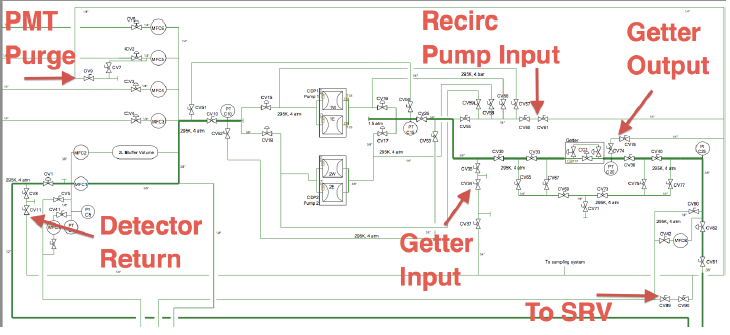
\includegraphics[width=150mm]{SamplingLocations.png}
\caption{Sampling Locations}
\label{fig:ports}
\end{figure}

\begin{figure}[h!]\centering
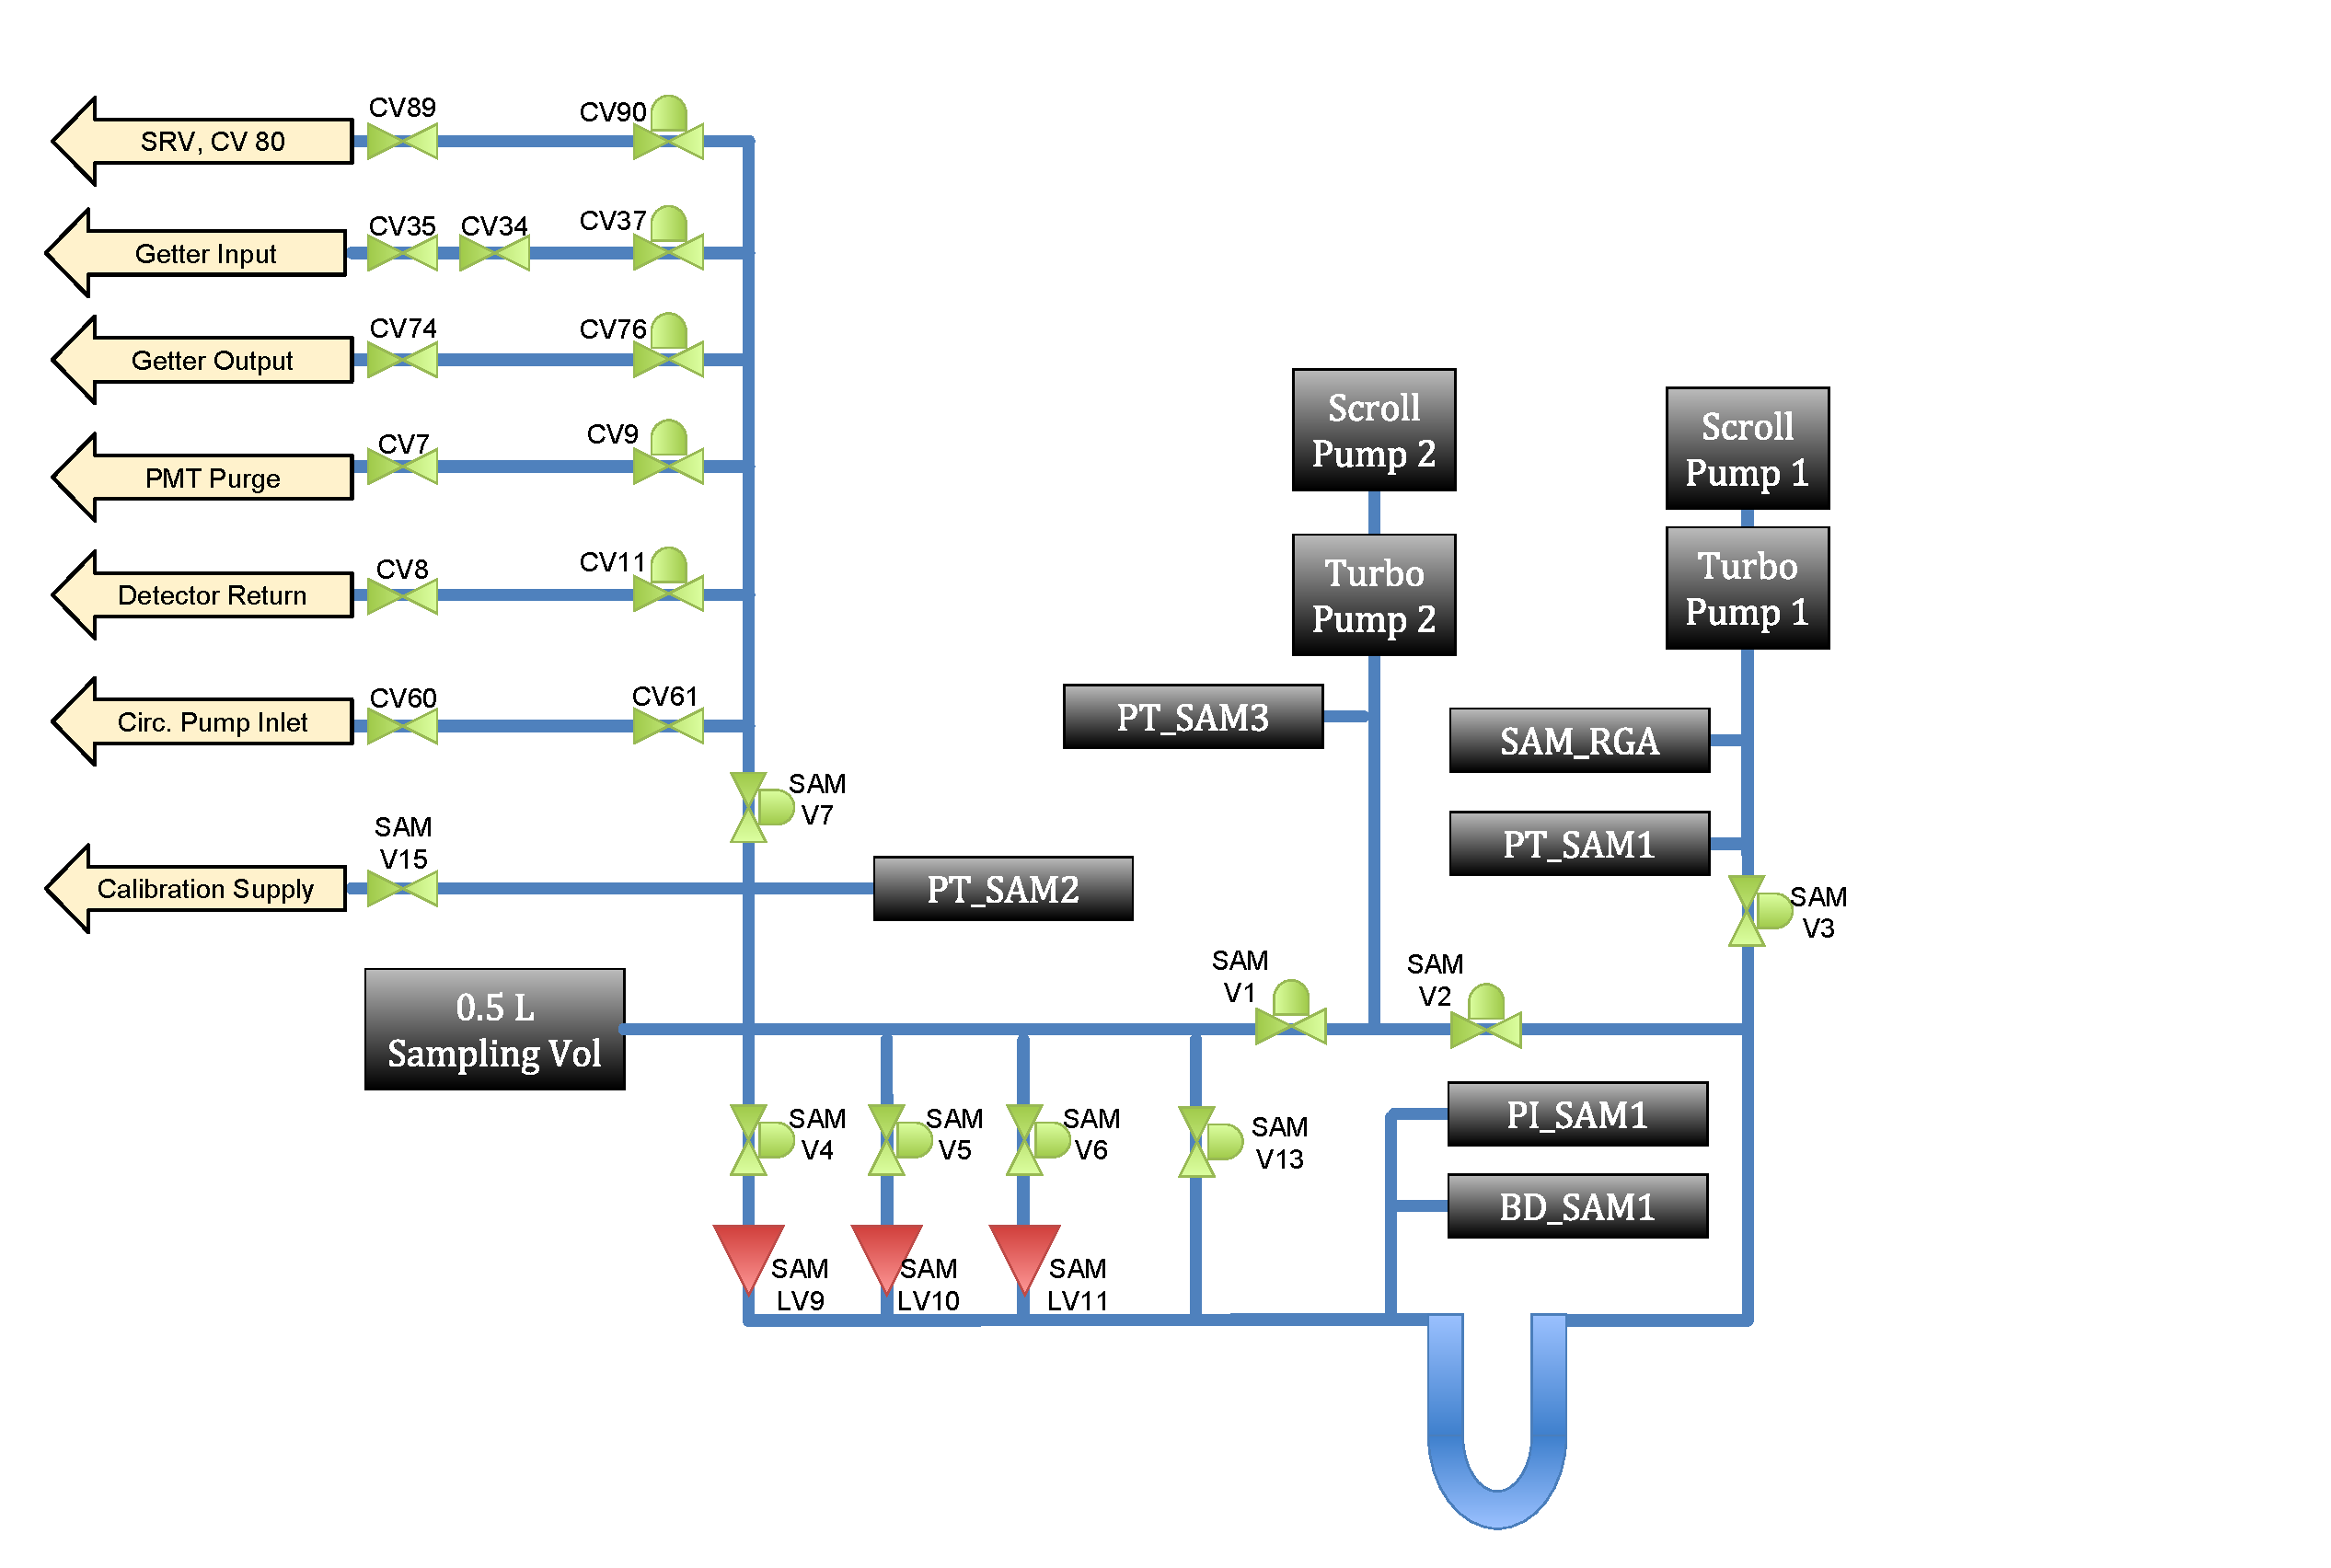
\includegraphics[width=150mm]{SAM_Diagram_3.pdf}
\caption{Diagram of the Coldtrap Sampling System}
\label{fig:pid}
\end{figure}

\begin{figure}[h!]\centering
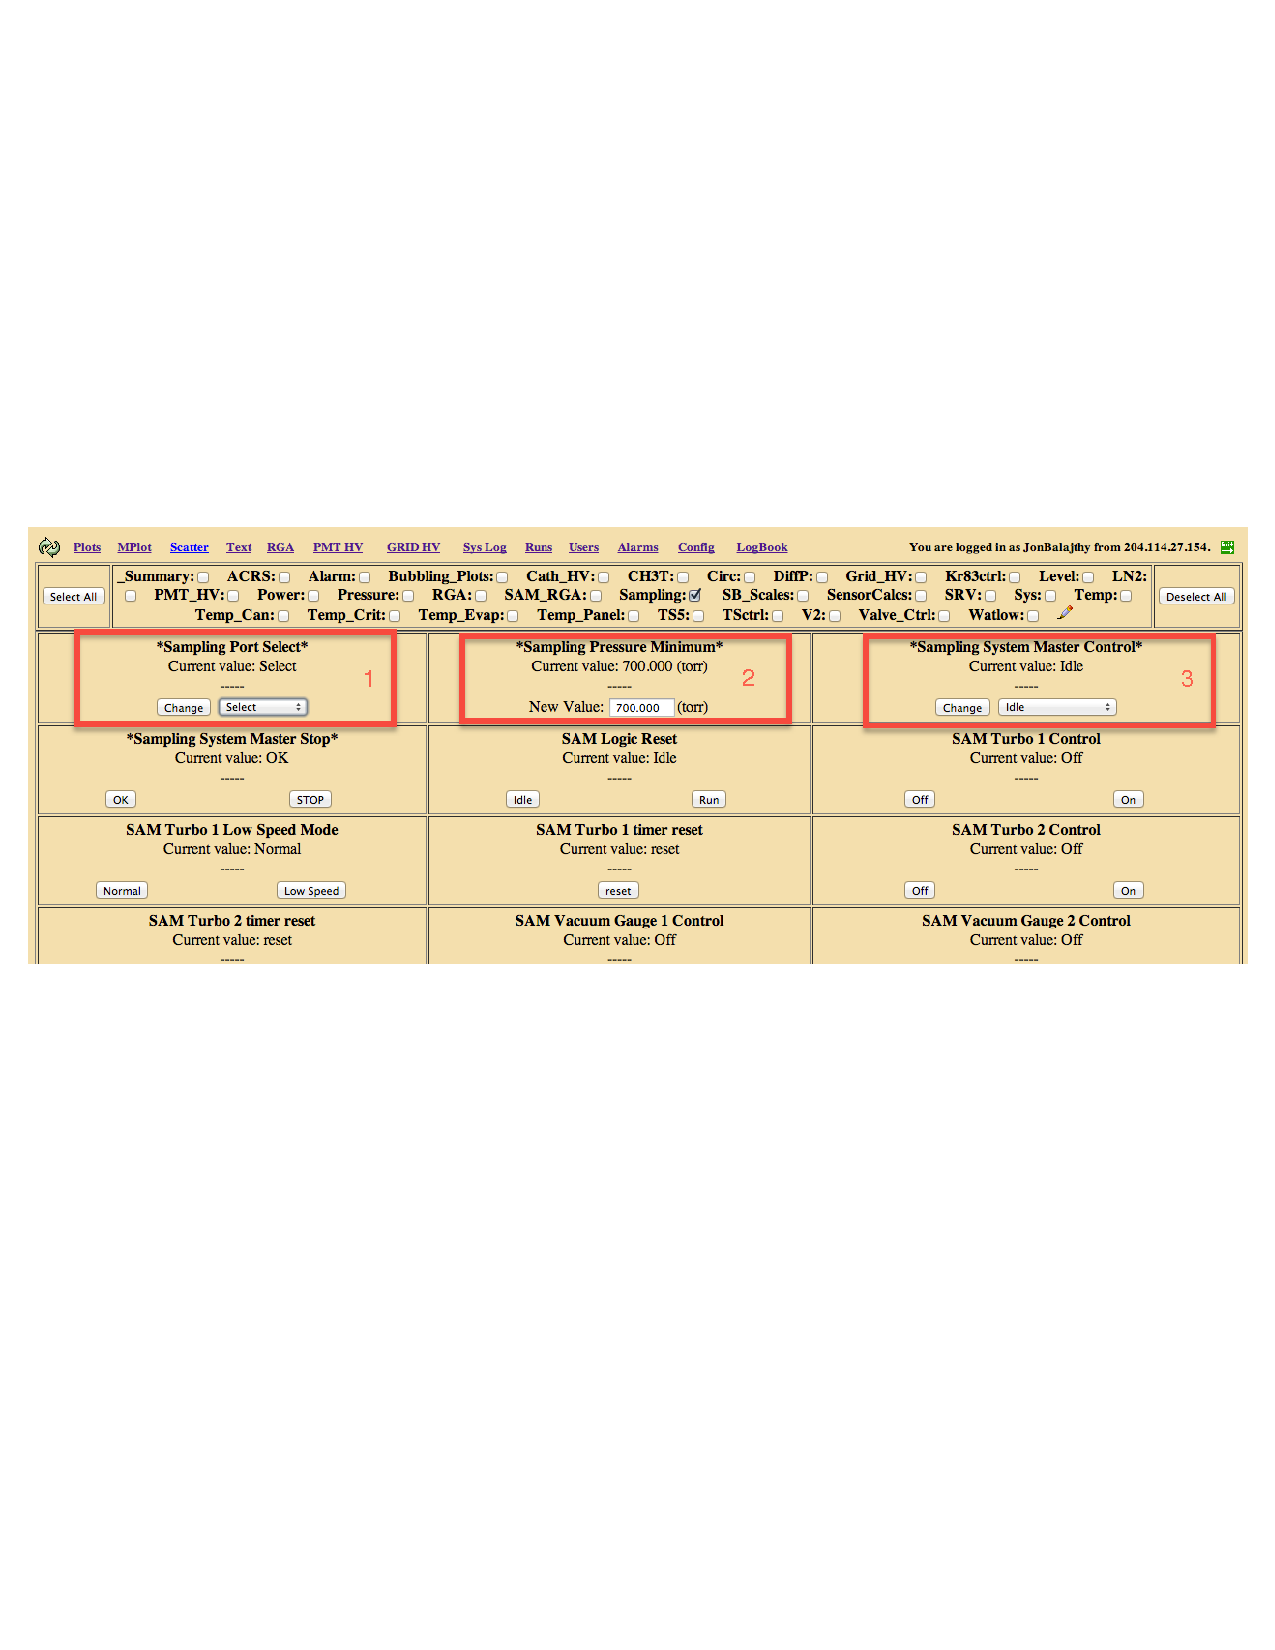
\includegraphics[width=180mm]{SAM_CTRL_2.pdf}
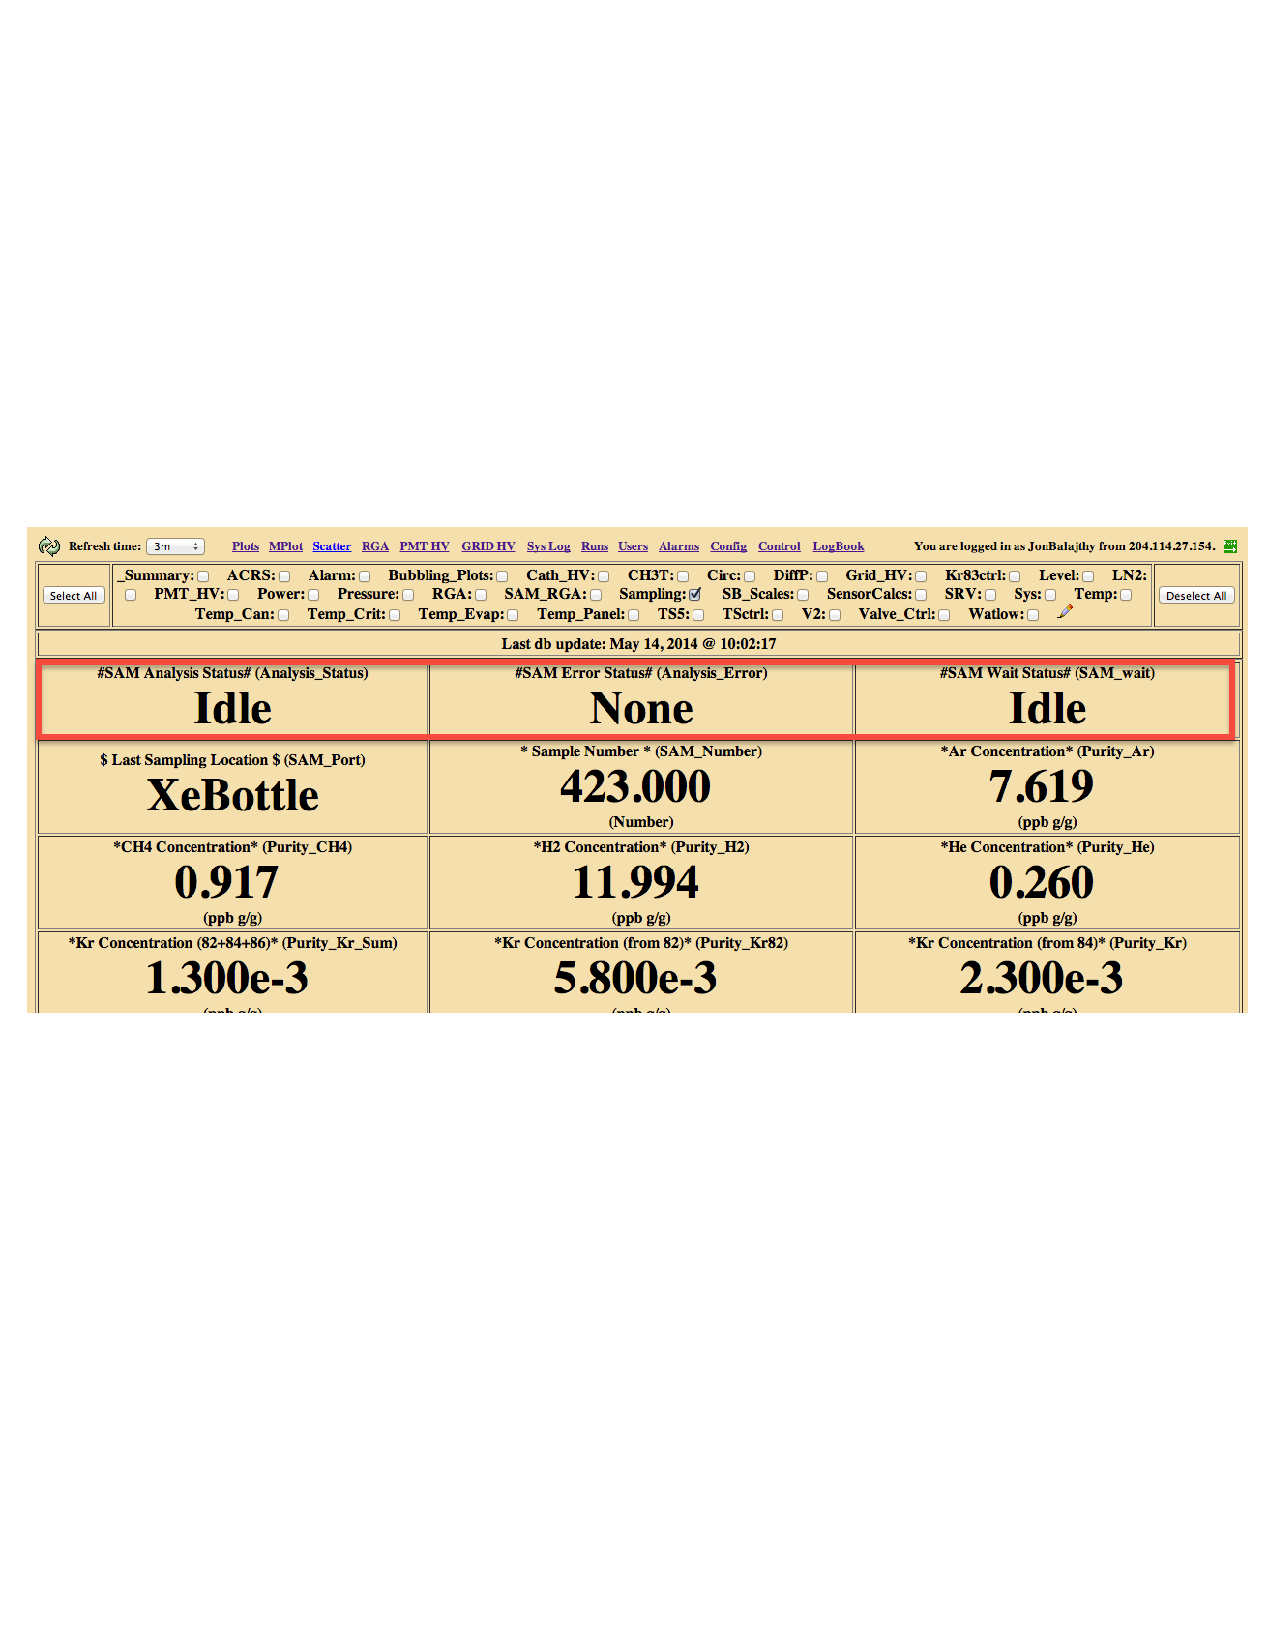
\includegraphics[width=180mm]{SAM_Status_2.pdf}
\caption{Top: The Sampling System Master Control box in LUX slow control. Bottom: The Sampling System status display in LUX slow control}
\label{fig:SC}
\end{figure}

\begin{figure}[h!]\centering
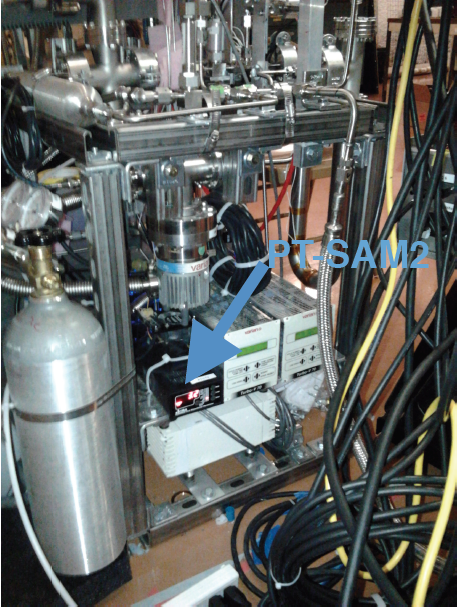
\includegraphics[width=100mm]{SAM.png}
\caption{The view of the sampling system from behind the circulation panel, where the xenon samples will be drawn. The user should watch PT-SAM2 when drawing a xenon sample.}
\label{fig:CM}
\end{figure}

\begin{figure}[h!]\centering
\includegraphics[width=110mm]{Min_Fill.pdf}
\caption{Minimum fill line on cold trap ``U"}
\label{fig:minfill}
\end{figure}


\begin{figure}[h!]\centering
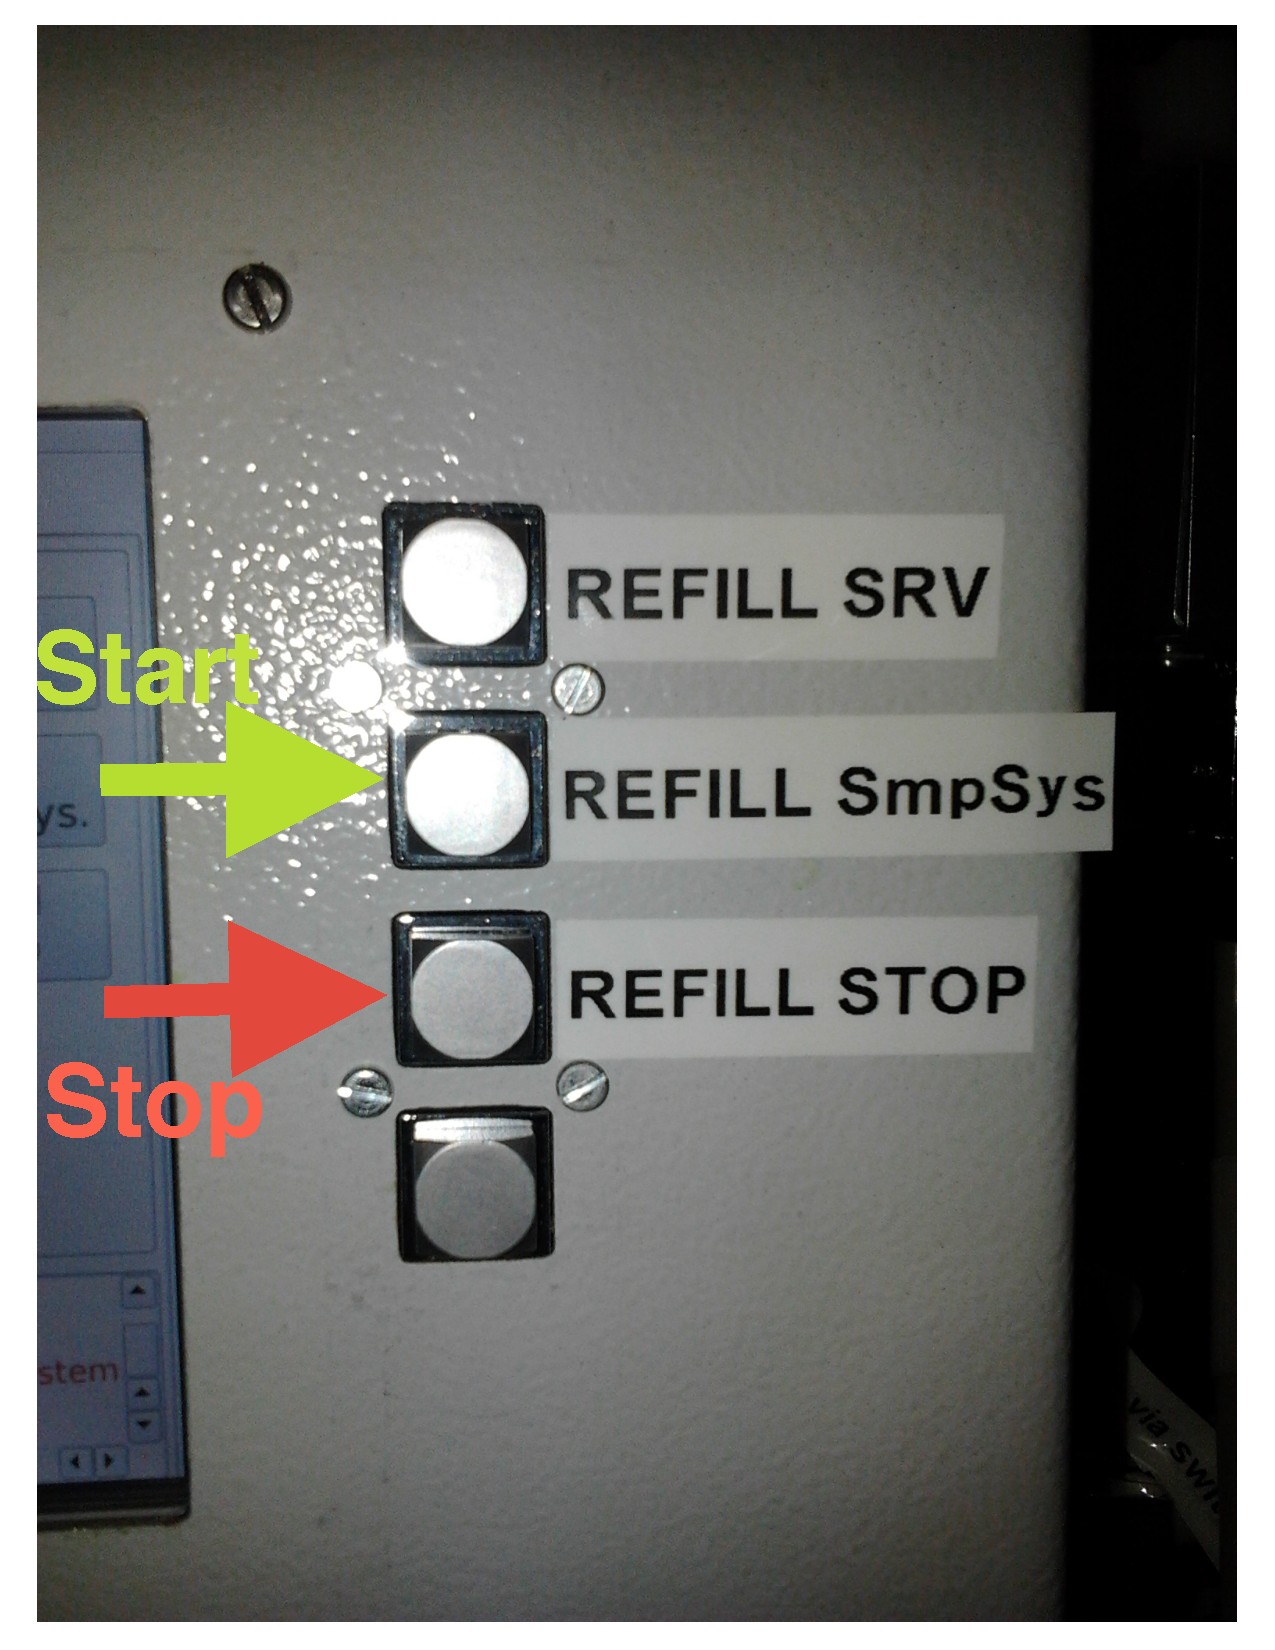
\includegraphics[width=100mm]{SRV_LN_BOX.pdf}
\caption{SRV LN system control box. To fill the 4 L transfer dewar push ``Refill SmsSys" to begin the flow of LN through the SRV pre-cool line. Once the dewar is full hit the ``Refill STOP" button.}
\label{fig:LN_BOX}
\end{figure}


\begin{figure}[h!]\centering
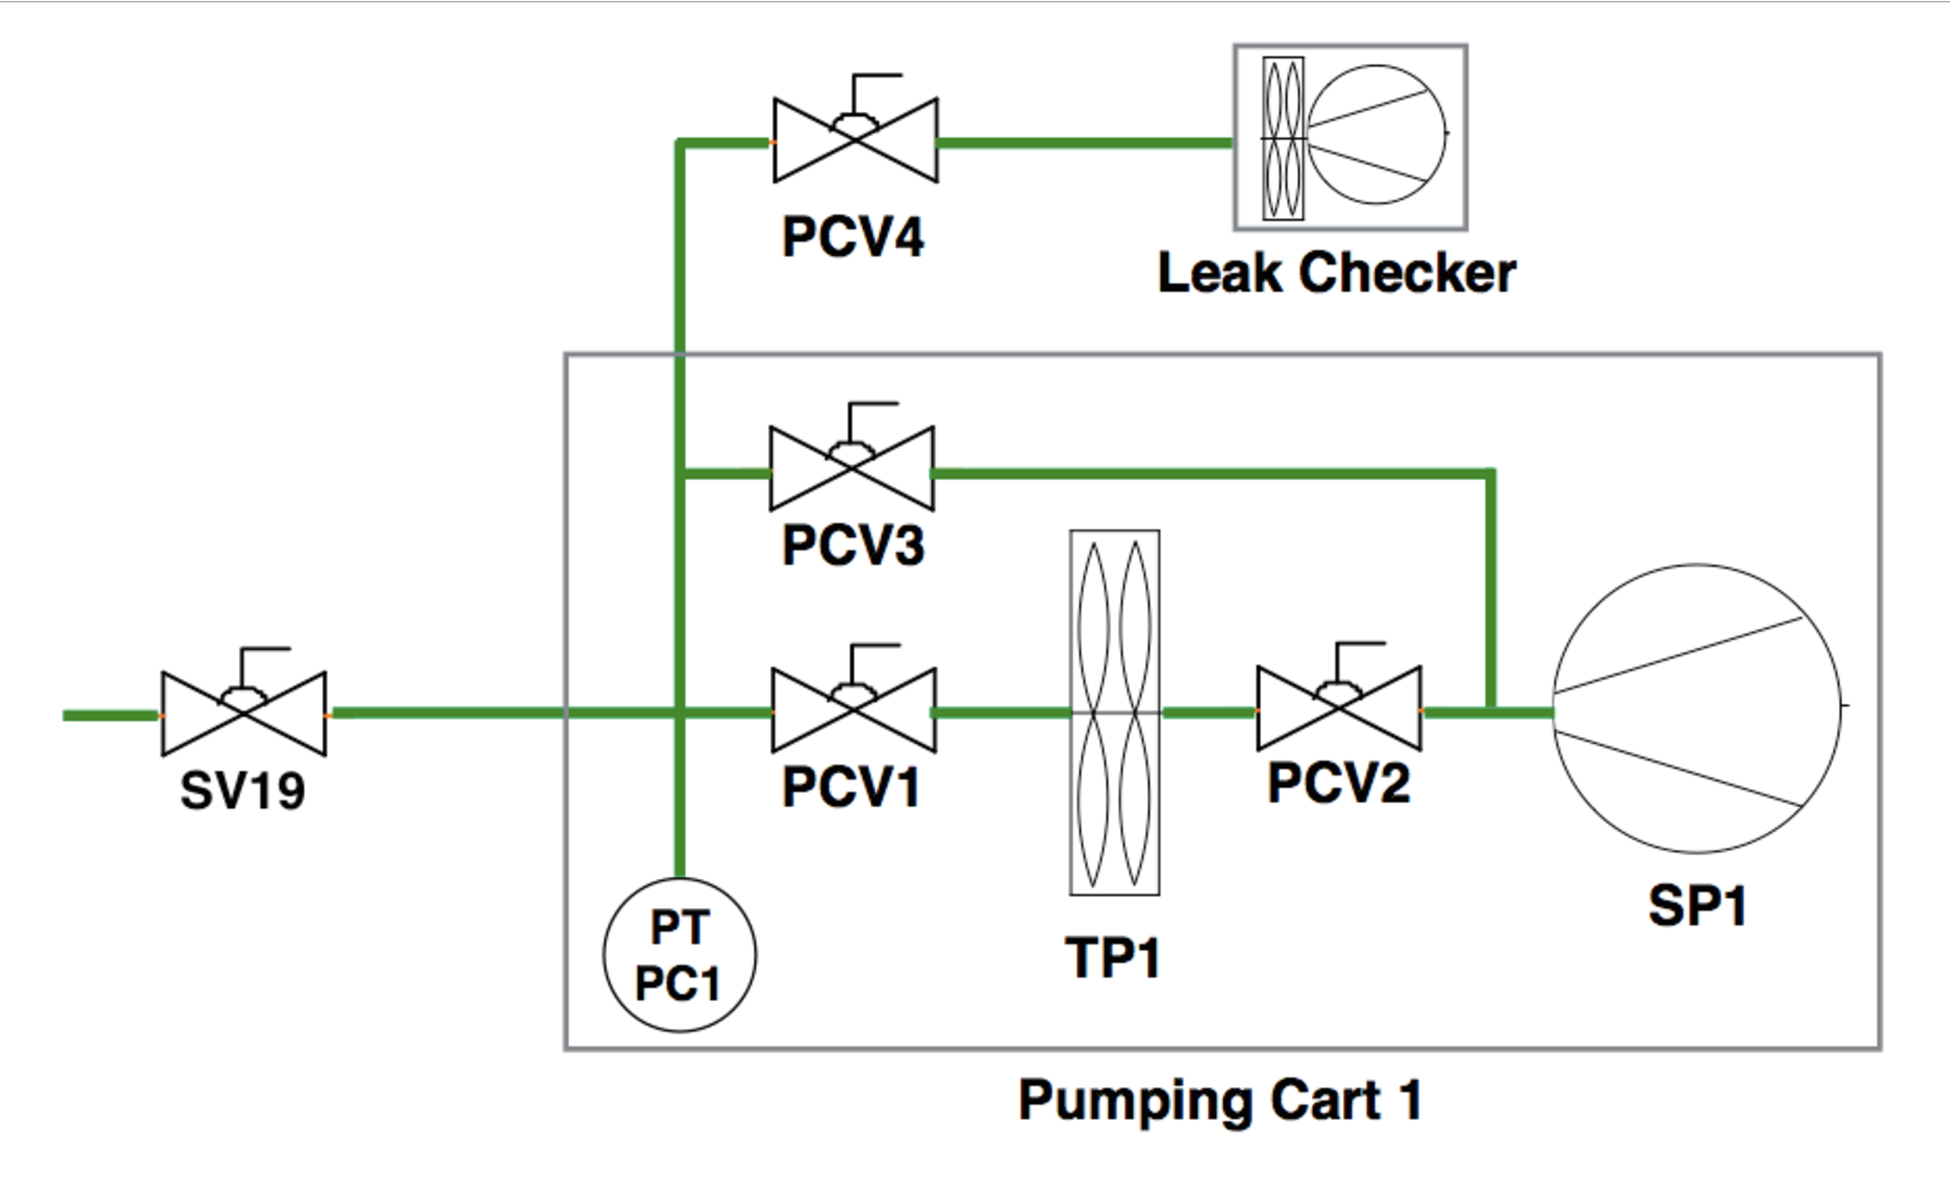
\includegraphics[width=130mm]{SAM_Turbo_Cart.pdf}
\caption{Diagram of the turbo pumping cart to be used when sampling LUX storage bottles in the bottle farm via SV19.}
\label{fig:TPC}
\end{figure}


\begin{figure}[h!]\centering
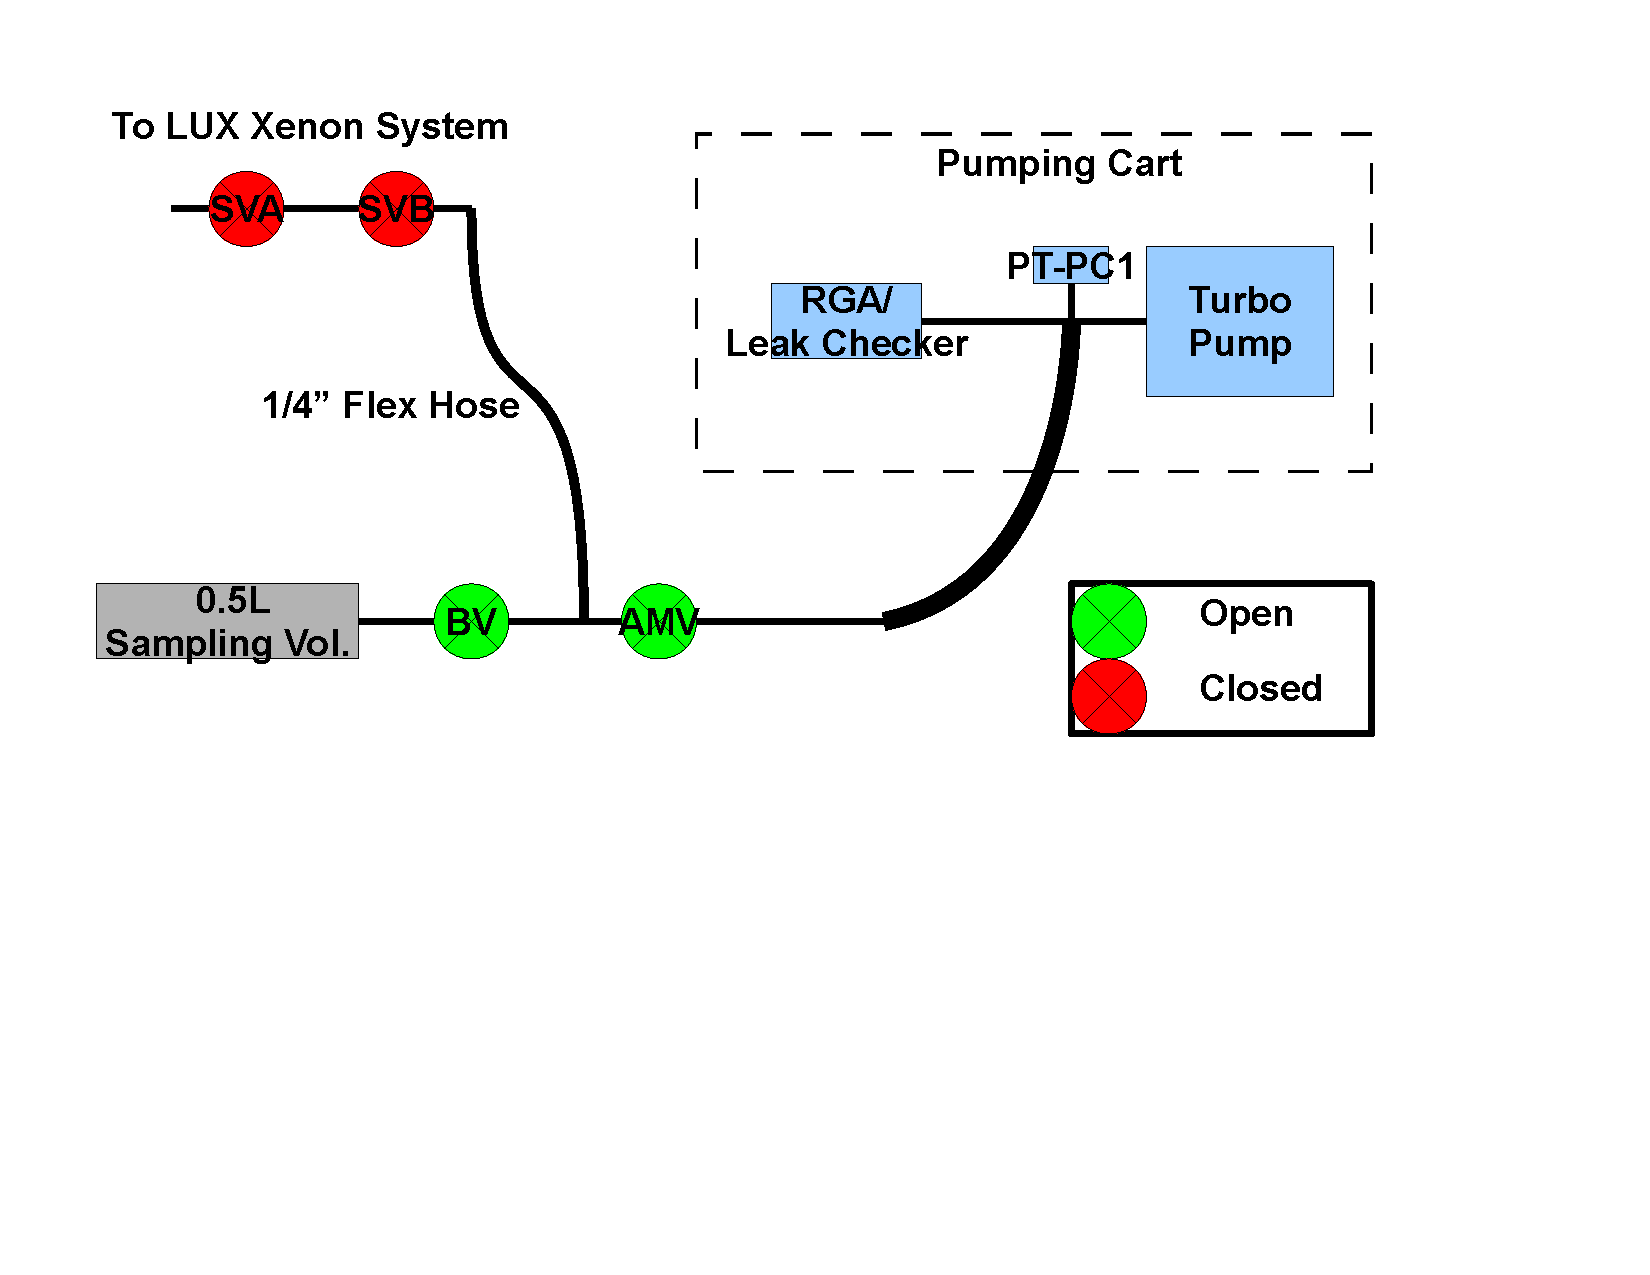
\includegraphics[width=150mm]{11.pdf}
\caption{Illustrated procedure for attaching the sampling manifold to the LUX xenon system}
\label{fig:fig2}
\end{figure}

\begin{figure}[h!]\centering
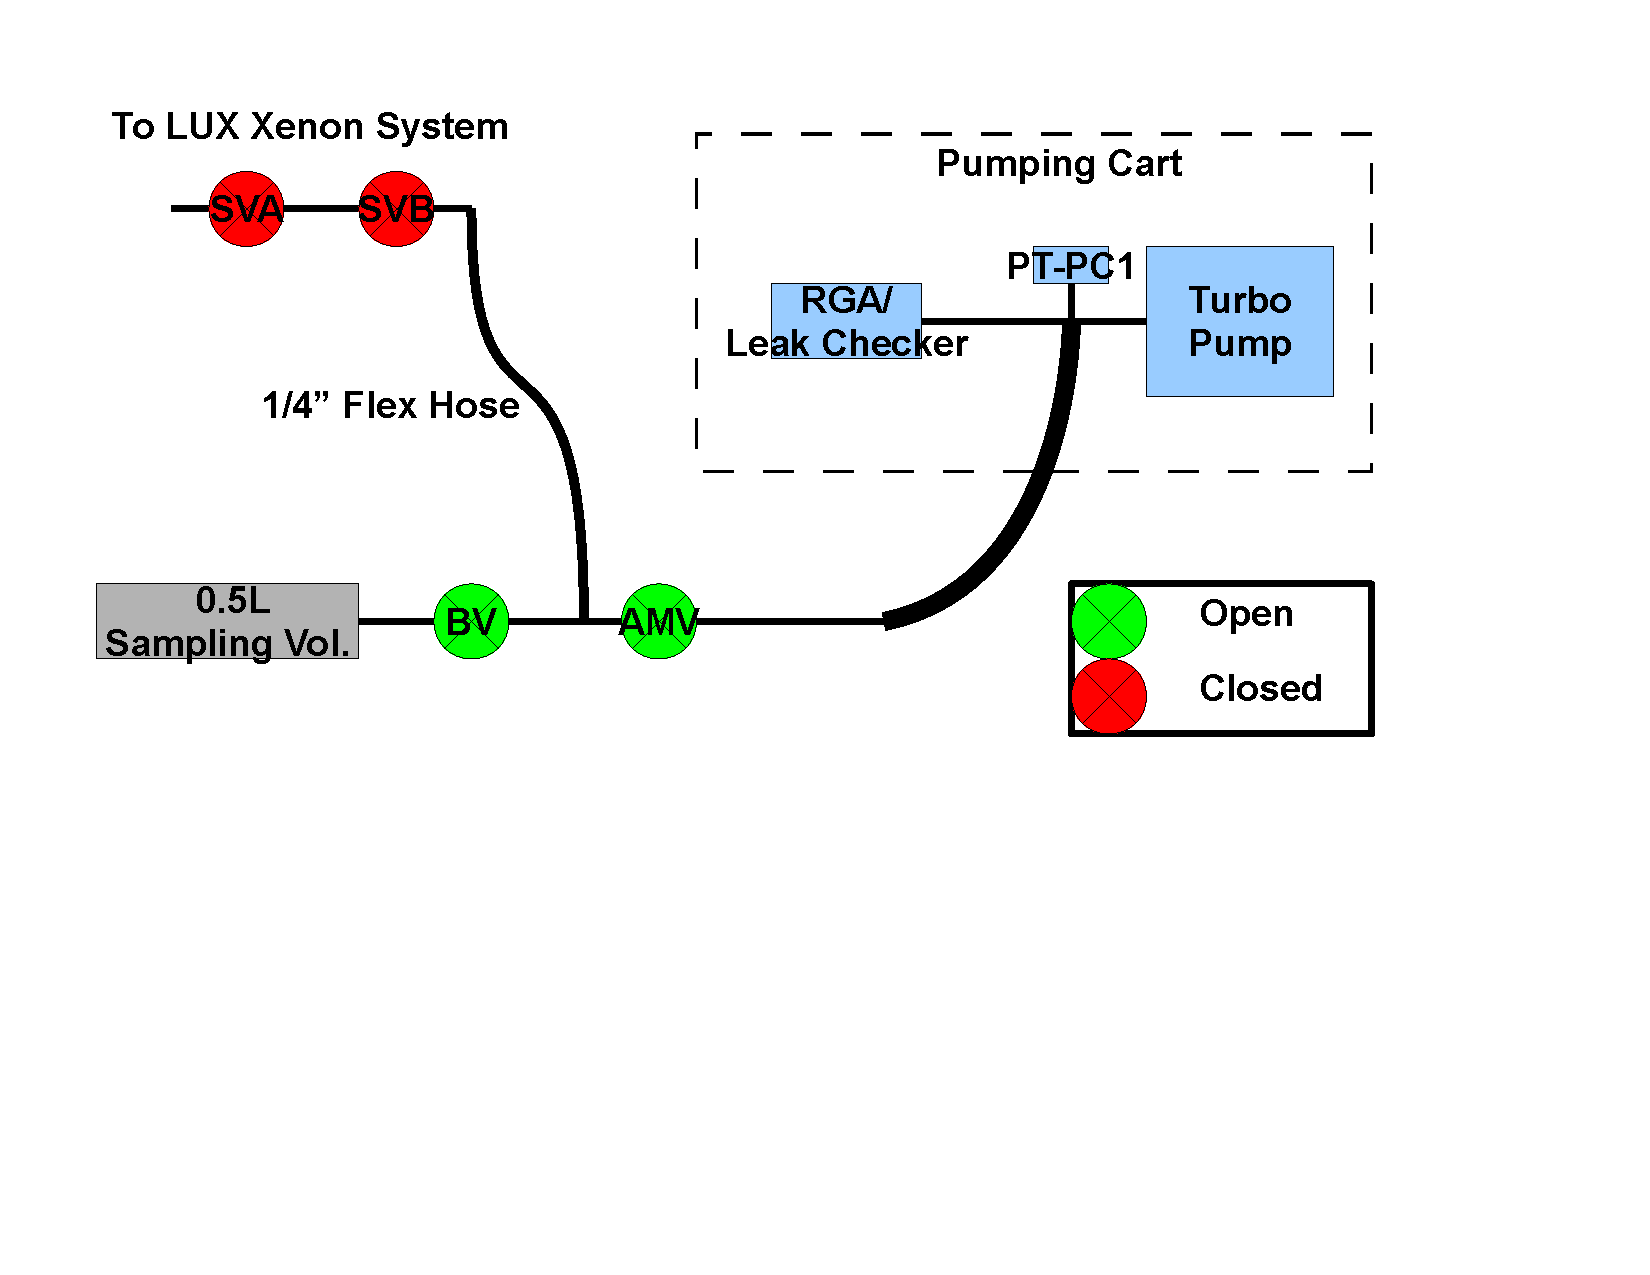
\includegraphics[width=80mm]{11.pdf}
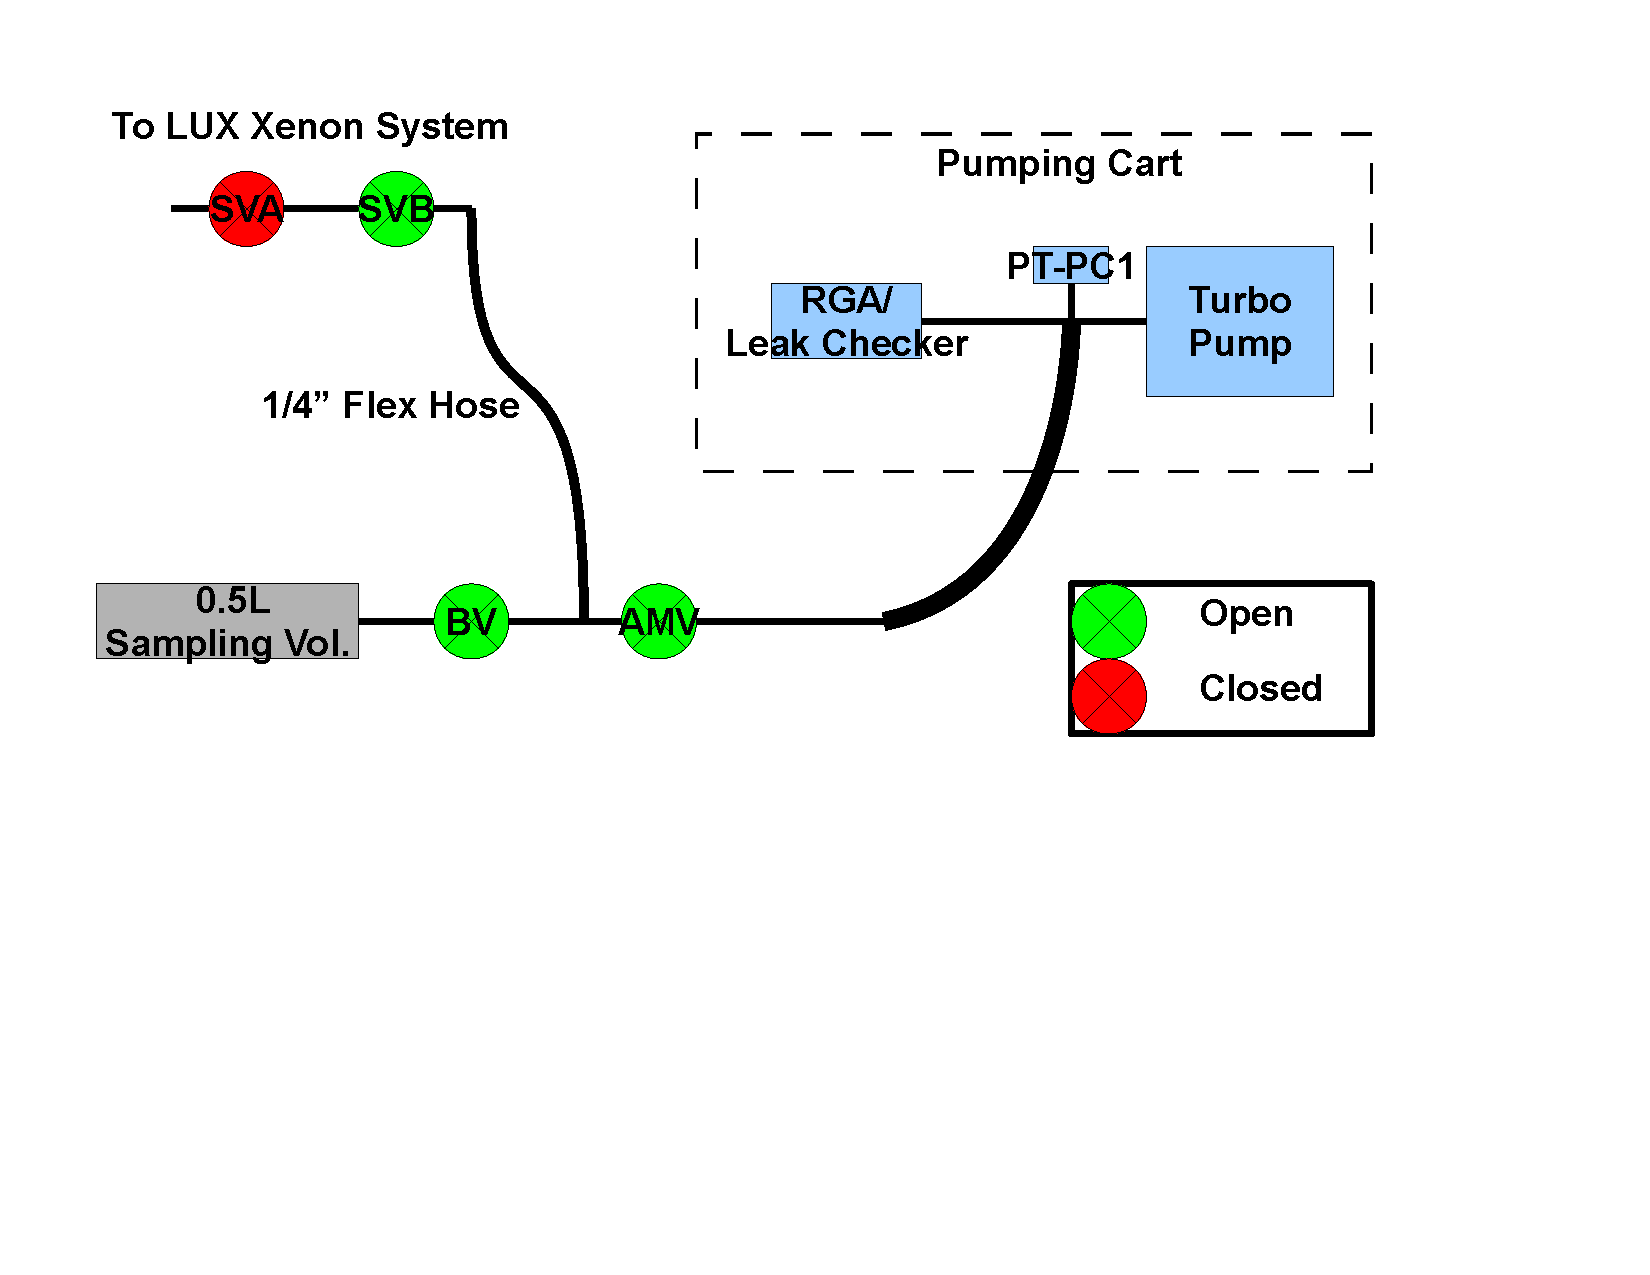
\includegraphics[width=80mm]{22.pdf}
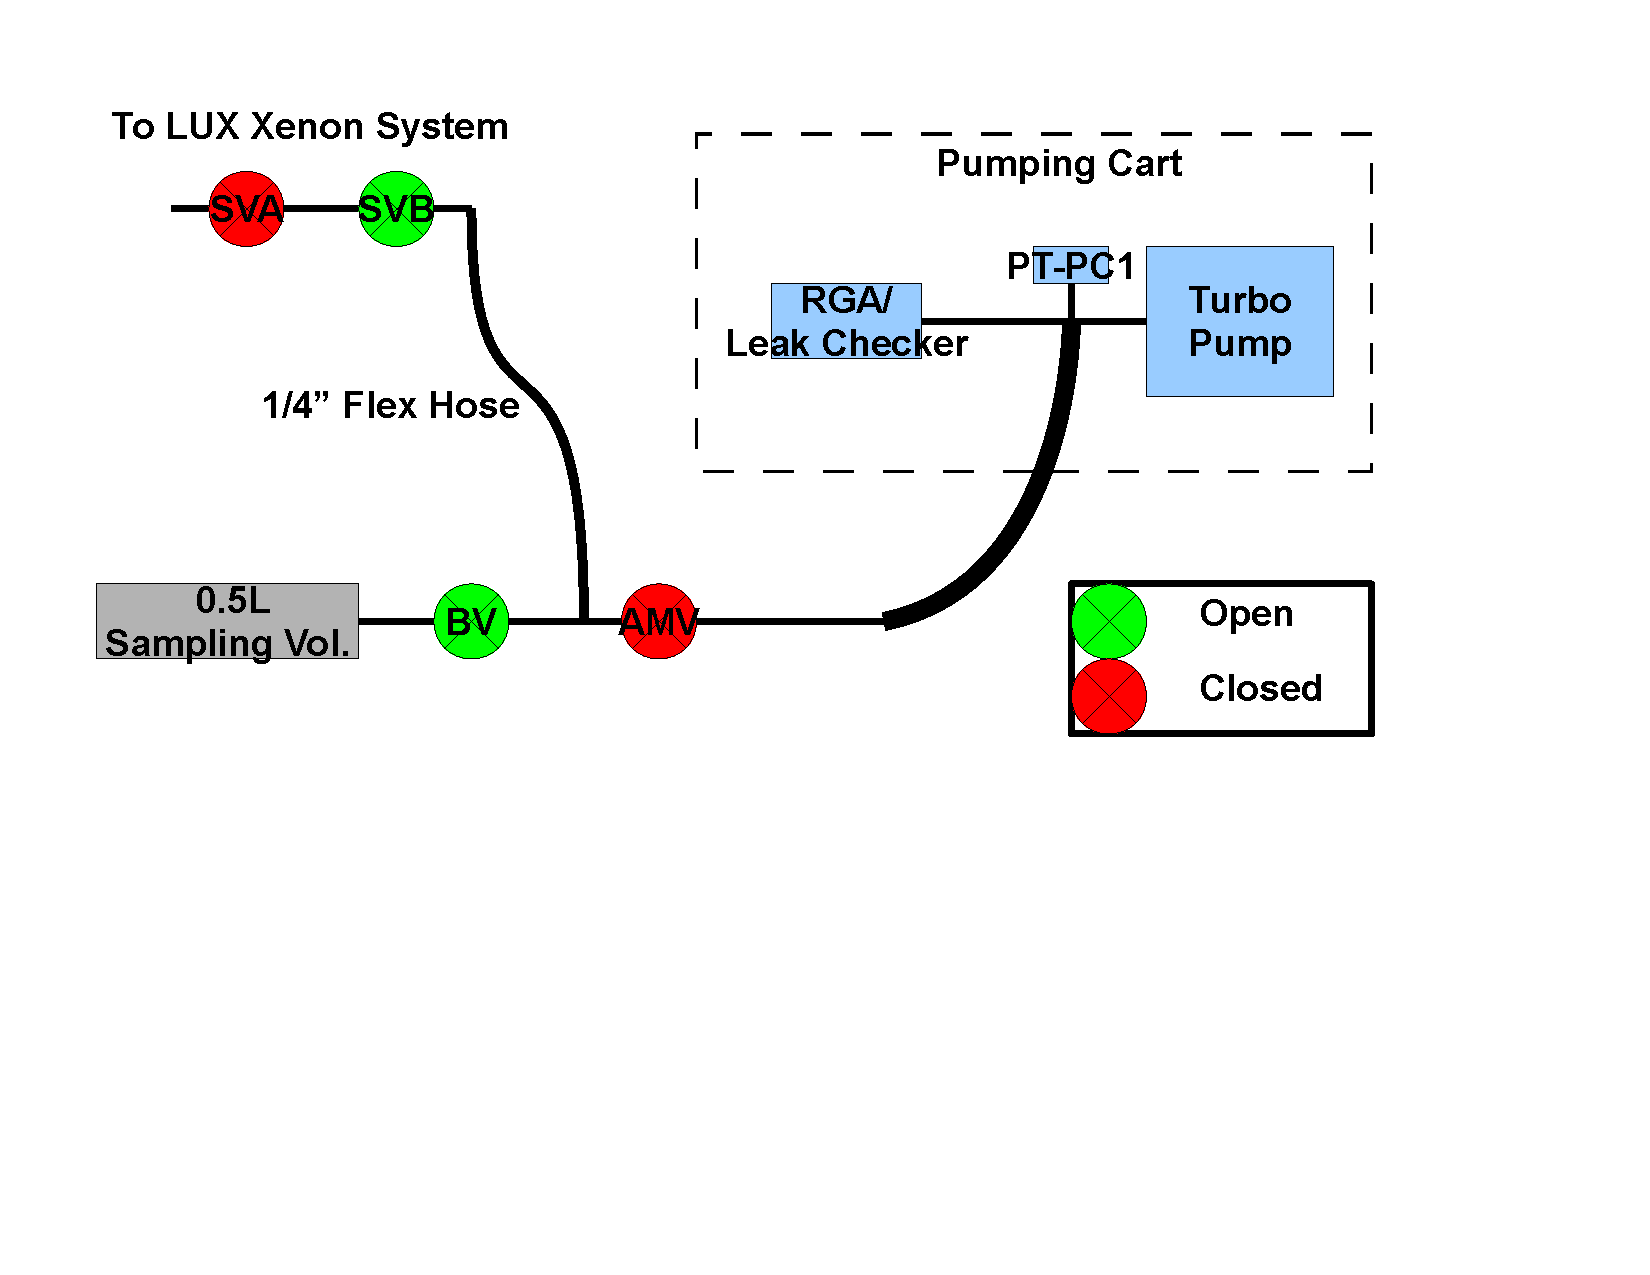
\includegraphics[width=80mm]{33.pdf}
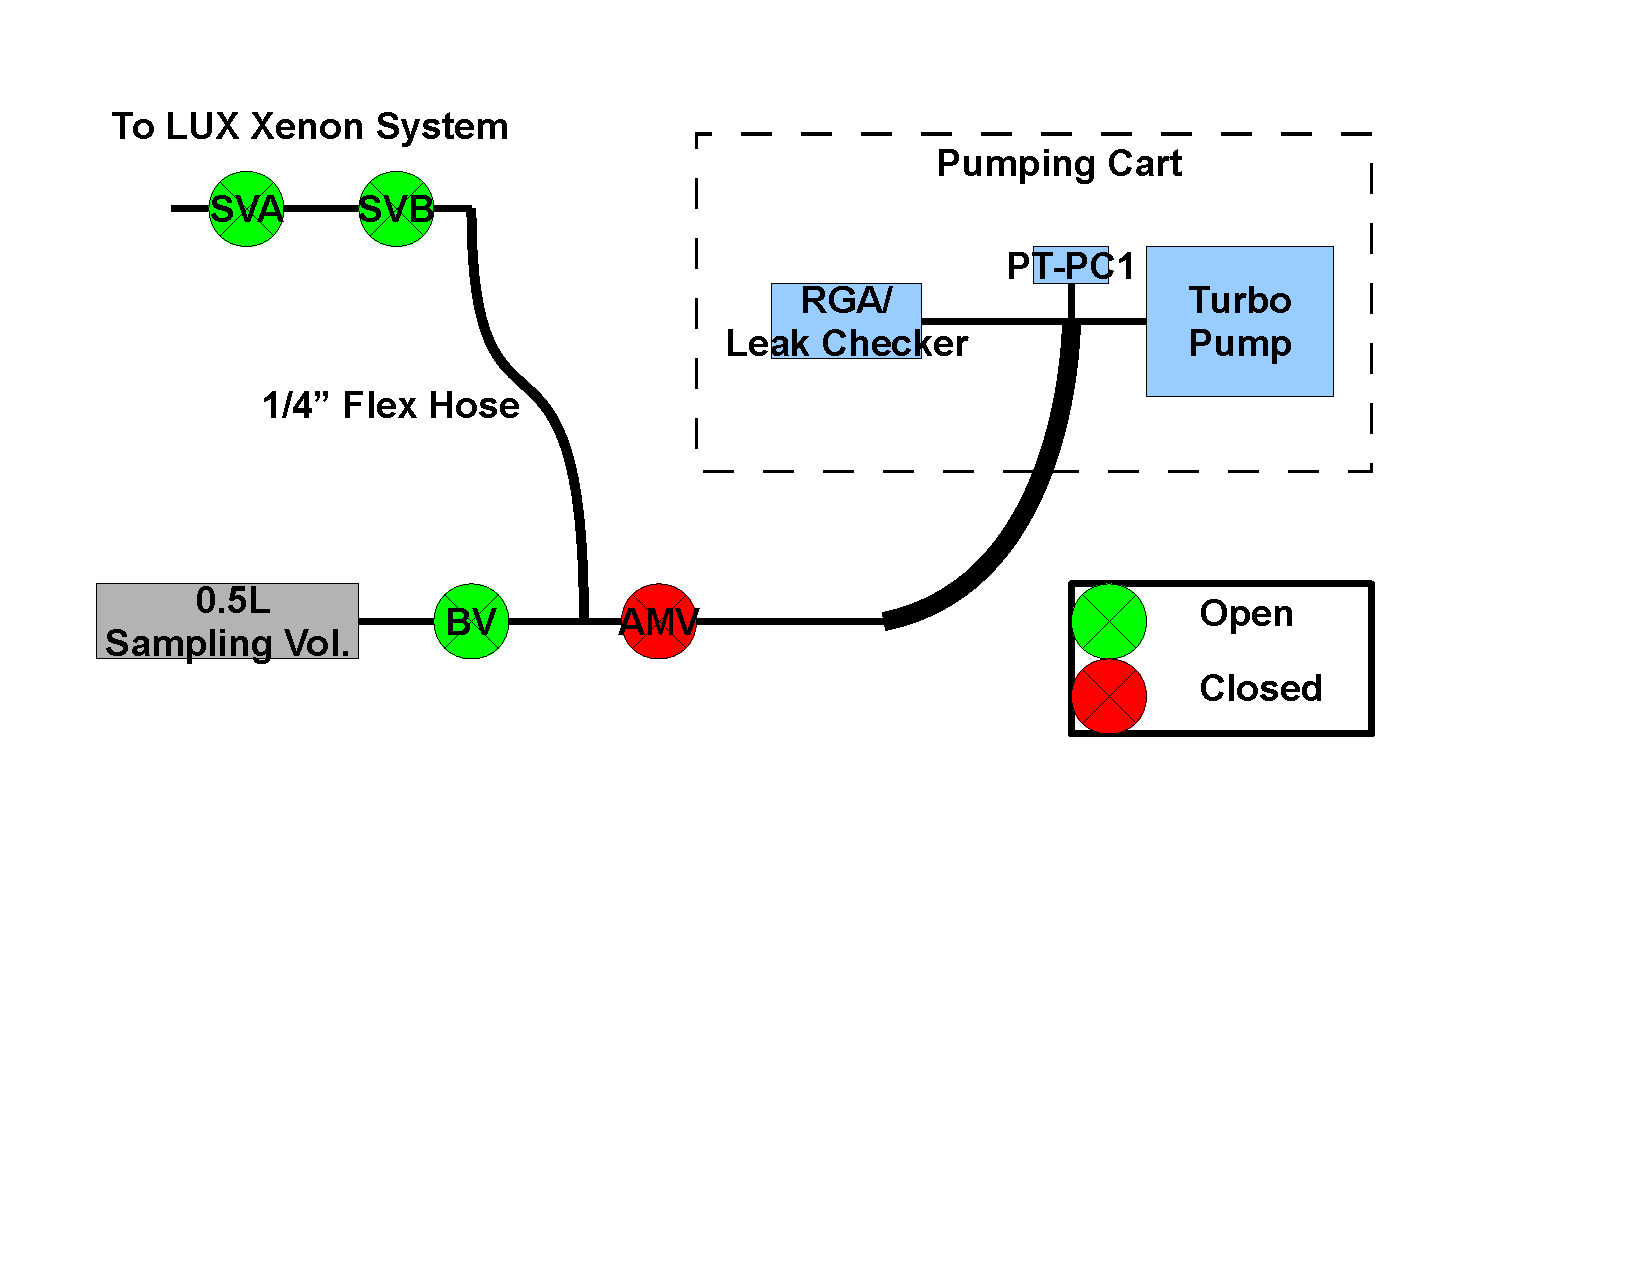
\includegraphics[width=80mm]{44.pdf}
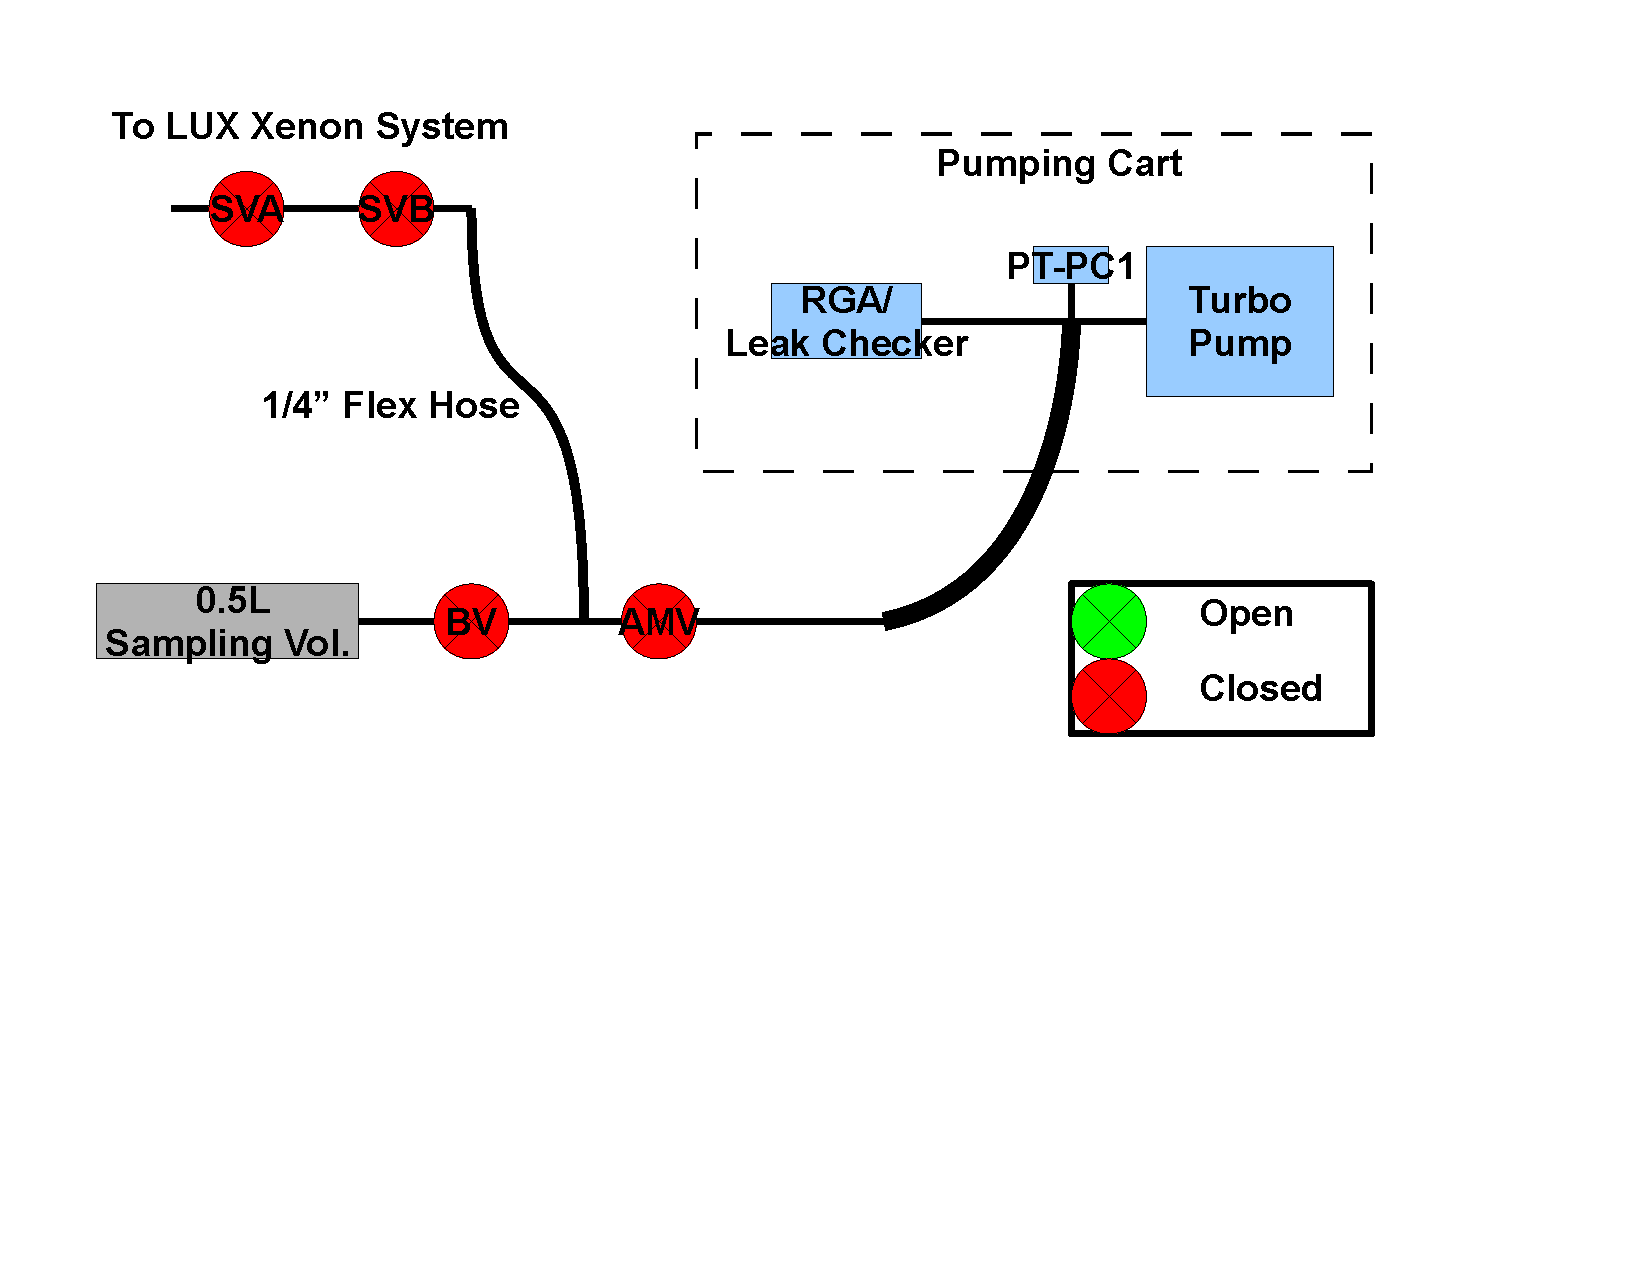
\includegraphics[width=80mm]{55.pdf}
\caption{Illustrated procedure for filling the sample bottle. First(top left), the sampling plumbing is attached to VB and then pumped to vacuum with the scroll-pump on the pumping cart. Second(top right), once the pressure on PT-PC1 reaches less than 0.1Torr VB is opened. The plumbing up to VA is then pumped to vacuum with the turbo-pump for one hour. Third(middle left), after pumping to vacuum for one hour the turbo-pump cart is isolated by closing AMV. Fourth(middle right), VA is opened filling the 0.5 L sample bottle with xenon at system pressure. Fifth(bottom), the VA, VB and the sample-bottle's valve (BV) are closed.}
\label{fig:steps}
\end{figure}




\end{document}
